\documentclass[11pt]{article}
\usepackage[margin=1in,a4paper]{geometry}
\usepackage[utf8]{inputenc}
\usepackage{hyperref}
\usepackage{amsmath,amssymb}
\usepackage{graphicx}
\usepackage{enumitem}
\usepackage[T1]{fontenc}
\usepackage[utf8]{inputenc}
\usepackage{cmap} 
\usepackage{inconsolata} 
\usepackage{xcolor}
\usepackage{listings}

% SETUP LISTINGS FOR R CODE CHUNKS
\lstset{
  language        = R,            % R syntax
  basicstyle      = \ttfamily\small, % single style for everything
  keywordstyle    = \color{blue},       % override coloured keywords
  commentstyle    = \color{gray},       % override coloured comments
  stringstyle     = \color{teal},       % override coloured strings
  frame           = single,      % box around
  numbers         = none,        % no line numbers
  keepspaces      = true,        % preserve your literal spaces
  columns         = fullflexible,% let TeX typeset each line as one run
  breaklines      = false,       % no auto-wrap (avoid extra line-runs)
  showstringspaces= false        % don’t mark spaces in strings
}

\setlist{nosep}  % compact list spacing
\begin{document}

\title{Actuarial Data Analytics I -- Subject Notes}
\author{Omar Amin}
\date{}
\maketitle

\tableofcontents

\newpage

\section{Overview of Statistical Learning and Data Analytics}
\subsection{What is Statistical Learning?}
Statistical learning refers to \textit{``a set of tools for making sense of complex datasets''}. In actuarial data analytics, these tools help us build models and algorithms to understand data and make predictions. Statistical learning encompasses both \textbf{supervised learning} and \textbf{unsupervised learning}: \\
\begin{itemize}
    \item \textbf{Supervised learning}: We have input variables (features) $X_1, X_2, \ldots, X_p$ and an output variable $Y$. The goal is to predict $Y$ or understand its relationship with $X$. If $Y$ is quantitative (numeric), it is a \textbf{regression} problem; if $Y$ is qualitative (categorical), it is a \textbf{classification} problem.
    \item \textbf{Unsupervised learning}: We only have features $X_1,\ldots,X_p$ and no explicit $Y$. The goal is to find patterns or groupings in the data without known responses. Examples include discovering clusters or underlying structure. 
\end{itemize} \phantom{i}

\noindent In supervised learning, the aim can be either \textbf{prediction} (accurately predicting unseen outcomes $Y$) or \textbf{inference} (understanding the effect of each $X_j$ on $Y$). We often split data into a \textbf{training set} and a \textbf{test set} to evaluate model performance on new data. A key concept is the \textbf{bias-variance trade-off}: as model flexibility increases, its bias tends to decrease but variance tends to increase. An optimal model achieves a good balance, minimizing the expected test error.

\subsection{Bias-Variance Trade-off and Model Accuracy}
\noindent A more restrictive model: more interpretable, easier for the inference goal. lasso $>$ linear models $>$ GAM, trees $>$ bagging, boosting. A more flexible model: better prediction accuracy, more complicated so harder to understand how each predictor behaves in the model. bagging, boosting $>$ GAM, trees $>$ linear models $>$ lasso. \\

\noindent The \textbf{training error} (error on the data used to fit the model) typically decreases as model complexity increases, but the \textbf{test error} (error on new data) follows a U-shape pattern. Initially, increasing flexibility reduces bias faster than it increases variance, so test error decreases; beyond a point, variance dominates and test error rises. This is why an overly complex model can overfit the training data and perform poorly on new data. In general higher flexibility $\implies$ higher variance and less bias. \\

\noindent We quantify prediction error as mean squared error for regression or mis-classification rate for classification. The lowest possible error is achieved by the theoretical \textbf{Bayes classifier} or function $f(x)$ (which we usually don't know). Our goal is to approximate this with a model $\hat f(x)$. The irreducible error (noise) sets a lower bound on what error we can achieve. \\

\noindent Key definitions:
\begin{itemize}
  \item \textbf{Bias}: error from erroneous assumptions in the learning algorithm. High bias means model is too simple to capture the true $f(x)$.
  \item \textbf{Variance}: error from sensitivity to small fluctuations in the training set. High variance means model is too complex (over fitting noise).
  \item \textbf{Mean Squared Error (MSE)} decomposition (for regression): $\mathbb{E}[ (Y - \hat f(X))^2 ] = (\text{Bias})^2 + \text{Variance} + \text{Irreducible Error}$. We seek to minimise bias+variance. $MSE = \frac{1}{n}\sum_{i=1}^{n}(y_i - \hat{f(\boldsymbol{x}_i)})^2$.
\end{itemize}

\newpage

\section{Linear/Multiple Linear Regression}
\subsection{Simple Linear Regression Theory}
Linear regression is a \textbf{supervised learning} method for predicting a quantitative response $Y$ based on one or more predictors $X_1,\ldots,X_p$. In \textbf{simple linear regression}, we have a single predictor $X$. The model assumes an approximate linear relationship:
\[ \hat Y = \beta_0 + \beta_1 X, \]
where $\beta_0$ is the intercept and $\beta_1$ is the slope. $\beta_1$ represents the expected change in $Y$ for a one-unit increase in $X$. The model is usually fit by \textbf{ordinary least squares (OLS)}, which finds $\hat\beta_0, \hat\beta_1$ that minimize the sum of squared residuals:
\[ \text{RSS} = \sum_{i=1}^n (y_i - \hat\beta_0 - \hat\beta_1 x_i)^2. \]

The solutions are:
\[ \hat\beta_1 = \frac{\sum_{i=1}^n (x_i - \bar{x})(y_i - \bar{y})}{\sum_{i=1}^n (x_i - \bar{x})^2}, \qquad 
\hat\beta_0 = \bar{y} - \hat\beta_1 \bar{x}, \] 
where $\bar{x}$ and $\bar{y}$ are the sample means. Key formulas:
\begin{itemize}
  \item \textbf{Predicted value:} $\hat{y}_i = \hat\beta_0 + \hat\beta_1 x_i$.
  \item \textbf{Residual:} $e_i = y_i - \hat{y}_i$.
  \item \textbf{Coefficient standard errors}: 
  $\operatorname{SE}(\hat\beta_1) = \sqrt{\frac{\sigma^2}{\sum (x_i-\bar{x})^2}}$, 
  and similarly for $\operatorname{SE}(\hat\beta_0) = \sigma \sqrt{\frac{1}{n}+\frac{\bar{x}^2}{\sum_{i=1}^{n}{(x_i - \bar{x})^2}}}$ (where $\sigma^2$ is estimated error variance).
  \item \textbf{R-squared ($R^2$) and RSE}: The proportion of variance in $Y$ explained by $X$: 
  $R^2 = 1 - \frac{\text{RSS}}{\text{TSS}}$, where $\text{TSS} = \sum (y_i-\bar{y})^2$. Also, Residual Standard Error (RSE) = $\sqrt{RSS/(n-2)}$. The $95\%$ CI for $\hat\beta_i$ is $\hat\beta_i \pm 1.96 \times \text{SE}(\hat\beta_i), \: i=0,1$.
\end{itemize} \phantom{i}

\noindent \textbf{Purpose and Description:} Linear regression models the relationship between $X$ and $Y$ with a line. It's easy to interpret: $\beta_1$ tells the direction and magnitude of effect of $X$ on $Y$. We can use it for prediction and to quantify relationships (with confidence intervals and hypothesis tests for $\beta_1$). \\

\noindent \textbf{Pros:} \\
\noindent Simple, interpretable, fast to fit, inference tools available (t-tests, etc.). Works well if true relationship is roughly linear and error terms are homoscedastic (equal variance).

\noindent \textbf{Cons:} \\
\noindent Only captures linear trends (unless extended), sensitive to outliers (which can drastically affect the slope), and performance degrades if relationship is non-linear or if there are important interaction effects not included. Violations of assumptions (e.g. non-constant variance, correlated errors) can invalidate inference.

\subsection{Simple Linear Regression in R (Example)}
We illustrate simple linear regression using the \texttt{Boston} housing dataset (from the \texttt{MASS} package). We predict median house value (\texttt{medv}) from proportion of low-status population (\texttt{lstat}). 

\begin{lstlisting}
# Load data and packages
library(MASS) # contains Boston dataset
data(Boston) # Boston housing data
# Fit a simple linear regression of medv on lstat
lm_fit <- lm(medv ~ lstat, data = Boston)
summary(lm_fit)
\end{lstlisting}

\noindent \textbf{Explanation:} We load the \texttt{MASS} library and the \texttt{Boston} dataset. The function \texttt{lm(medv ~ lstat, data=Boston)} fits a linear model $\text{medv} = \beta_0 + \beta_1 \text{lstat} + \epsilon$. The result \texttt{lm\_fit} contains the fitted coefficients and other information. \texttt{summary(lm\_fit)} prints the model summary, including estimates $\hat\beta_0, \hat\beta_1$, their standard errors, $t$-statistics and $p$-values (testing $H_0: \beta_j=0$), $R^2$, etc. For example, output might show:

\begin{verbatim}
Coefficients:
            Estimate Std. Error t value Pr(>|t|)    
(Intercept) 34.5538    0.5627   61.42   <2e-16 ***
lstat       -0.9505    0.0387  -24.57   <2e-16 ***
\end{verbatim}

This indicates $\hat\beta_0 \approx 34.55$ and $\hat\beta_1 \approx -0.95$. So the fitted equation is $\widehat{\text{medv}} = 34.55 - 0.95 \times \text{lstat}$. The negative slope implies that higher \texttt{lstat} (more low-status population) is associated with lower median home value. The $p$-value is $<2e-16$, indicating the relationship is statistically significant. \\

\noindent We can also obtain the coefficients directly with \texttt{coef(lm\_fit)} or confidence intervals for them using \texttt{confint(lm\_fit)}.

To visualise the fit:
\begin{lstlisting}
plot(Boston$lstat, Boston$medv, col="blue",
     main="Linear Fit: medv vs lstat", 
     xlab="% Low Status (lstat)", ylab="Median Value (medv)")
abline(lm_fit, col="red", lwd=2)
\end{lstlisting}

\noindnt This produces a scatterplot of the data and overlays the regression line in red. \\

\noindent \textbf{Interpreting the model:} For a 1\% increase in \texttt{lstat}, the model predicts a decrease of about $0.95$ in \texttt{medv} (in thousands of dollars). The intercept 34.55 is the predicted \texttt{medv} when \texttt{lstat}=0 (extrapolated baseline). The $R^2$ (about 0.544) tells us ~54.4\% of the variance in home value is explained by \texttt{lstat} in this simple linear model.

\subsection{Multiple Linear Regression Theory}
Multiple linear regression generalizes to $p$ predictors. The model:
\[ Y = \beta_0 + \beta_1 X_1 + \cdots + \beta_p X_p + \varepsilon, \]
fitted by least squares minimizing $\text{RSS} = \sum_{i=1}^n (y_i - \hat\beta_0 - \hat{\beta}_1x_{i1} + ... + \hat\beta_px_{ip})^2$. Interpretation of coefficients: $\beta_j$ is the expected change in $Y$ for a one-unit increase in $X_j$, holding all other predictors fixed. \\

\noindent Important considerations:
\begin{itemize}
  \item \textbf{t-tests}: We test $H_0:\beta_j=0$ for each coefficient (given others in model). A small $p$-value indicates predictor $X_j$ contributes significantly (after accounting for others).
  \item \textbf{F-test}: A global test whether at least one $\beta_j \neq 0$. It compares the full model to the intercept-only model (answers if atleast one of hte predictors are useful in predicting the response).
  \item \textbf{Dummy variables}: Qualitative predictors are incorporated via dummy (indicator) variables. For example, a categorical variable with $k$ classes is encoded with $k-1$ dummy binary variables.
  \item \textbf{Interactions}: We can include interaction terms (e.g. $X_1 \times X_2$) to allow the effect of one predictor to depend on another.
  \item \textbf{Model fit}: $R^2$ still indicates proportion of variance explained (it always increases when adding predictors). Adjusted $R^2$ penalizes adding useless predictors.
\end{itemize}

\noindent \textbf{Pros:} \\
\noindent Captures linear effects of multiple variables, enabling control for confounders. Inference allows testing each predictor’s effect. The model is easy to implement and interpret (coefficients as marginal effects).

\noindent \textbf{Cons:} \\
\noindent Still assumes linear form, which may be too restrictive. Sensitive to multicollinearity (high correlation among predictors can inflate standard errors and make coefficient estimates unstable). Outliers or high-leverage points can distort the fit. If $p$ is large relative to $n$, overfitting can occur.

\subsection{Multiple Linear Regression in R (Example)}
Using the Boston data, suppose we include two predictors, \texttt{lstat} and \texttt{age}, to predict \texttt{medv}:
\begin{verbatim}
lm_fit2 <- lm(medv ~ lstat + age, data = Boston)
summary(lm_fit2)
\end{verbatim}
This fits $\widehat{\text{medv}} = \beta_0 + \beta_1 \text{lstat} + \beta_2 \text{age}$. The summary might show:
\begin{verbatim}
Coefficients:
            Estimate Std. Error t value Pr(>|t|)    
(Intercept) 33.2228   0.73085   45.46   <2e-16 ***
lstat       -1.0321   0.04819  -21.42   <2e-16 ***
age          0.0345   0.01223    2.82   0.005 <**
\end{verbatim}
This suggests both \texttt{lstat} and \texttt{age} have significant effects. Interestingly, $\hat\beta_2$ (age) is positive (older homes associated with slightly higher value, controlling for lstat). Note that the coefficient of \texttt{lstat} ($-1.03$) is a bit different than in the simple regression ($-0.95$) because now it represents the effect of \texttt{lstat} holding \texttt{age} fixed.

We can include all predictors using \texttt{medv ~ .} formula:
\begin{verbatim}
lm_fit_full <- lm(medv ~ ., data = Boston)  # all 13 predictors
summary(lm_fit_full)
\end{verbatim}
This yields a full model with all variables. We could then perform variable selection (discussed in Week 4) to simplify the model if needed. \\

\noindent \textbf{Diagnostics:} We can examine diagnostic plots for linear regression:
\begin{verbatim}
par(mfrow=c(2,2))
plot(lm_fit_full)
\end{verbatim}
This produces residual plots, Q-Q plot for residuals, scale-location plot, and leverage plot. We look for non-linear patterns (indicating model mis-specification), non-constant variance, outliers, or high leverage points. 

\subsection{Polynomial Regression and Model Flexibility}
Often the linearity assumption is too restrictive. One way to model a non-linear relationship is to include transformations of predictors. \textbf{Polynomial regression} adds polynomial terms. For example, a quadratic model:
\[ Y = \beta_0 + \beta_1 X + \beta_2 X^2 + \varepsilon, \] 
can capture curvature. Higher-degree polynomials (cubic, quartic, etc.) provide more flexibility. \\

\noindent In R, we can use \texttt{poly()} or the $I()$ function to include polynomial terms. For example:
\begin{verbatim}
lm_poly4 <- lm(medv ~ poly(lstat, 4), data=Boston)
\end{verbatim}
fits a 4th-degree polynomial in \texttt{lstat}. Alternatively:
\begin{verbatim}
lm_poly4_raw <- lm(medv ~ lstat + I(lstat^2) + I(lstat^3) + I(lstat^4),
                   data=Boston)
\end{verbatim}
includes powers of \texttt{lstat} explicitly (using $I()$ to inhibit formula interpretation). Polynomial terms are just one form of basis functions; others include piecewise polynomials and splines. \\

\noindent Including polynomial terms increases model flexibility (reduces bias) but also risk of overfitting (increased variance). One can use cross-validation (see below) to select the polynomial degree that optimizes test error. \\

\newpage

\section{Resampling Methods}

\noindent \textbf{Resampling methods} like cross-validation help determine model complexity. They do not create new models but provide a way to assess a given model’s performance on unseen data. \\

\subsection{Validation Set Approach}
\noindent Randomly dividing the available set of observations into two parts, a \textit{training set} and a \textit{validation set}. The model is fit on the training set, and the fitted model is used to predict the response for the observations in the validation set. \\

\noindent Potential drawbacks:
\begin{itemize}
    \item The validation estimate of the test error rate can be highly variable.
    \item Only a subset of the observations are used to fit the model. Therefore, the validation set error rate may tend to overestimate the test error rate for the model fit on the entire data set.
\end{itemize}

\subsection{Leave-One-Out Cross Validation (LOOCV)}
\noindent Involves splitting the set of observations into two parts, but with the validation set only containing a single observation. \\

\begin{enumerate}
    \item Using the observation $(x_1, y_1)$ as the validation set and $\{ (x_2,y_2),...,(x_n,y_n) \}$ as the training set to fit a model that generates a prediction $\hat y_1$ by $x_1$. Then $MSE_1 = (y_1 - \hat y_1)^2$.
    \item Using observation $(x_2,y_2)$ as the validation set and $\{ (x_1,y_1),(x_3,y_3),...,(x_n,y_n) \}$ as the training set to fit a model that generates a prediction $\hat y_2$ by $x_2$. Then $MSE_2 = (y_2 - \hat y_2)^2$.
    \item Repeat this by selecting every remaining observation as the validation observation and obtain $MSE_3,...,MSE_n$.
    \item The LOOCV estiamte for the test MSE is then $CV_{(n)} = \frac{1}{n}\sum_{i=1}^{n}{MSE_i}$. If $n$ is large, this process is very time consuming.
\end{enumerate} \phantom{i}

\noindent \textbf{Advantages of LOOCV}:
\begin{itemize}
    \item LOOCV has much less bias than the validation set approach, since when fitting the method the training sets almost cover the whole data set. So, LOOCV tends not to overestimate the test error rate.
    \item Validation set approach will yield different results when applied repeatedly. Performing LOOCV multiple times will always yield the same results, so no randomness.
    \item For least squares linear or polynomial regression, there is a computational shortcut. $CV_{(n)} = \frac{1}{n}\sum_{i=1}^{n}\Big( \frac{y_i - \hat y_i}{1 - h_i} \Big)^2$. $h_i$ is the leverage statistic. In simple linear regression: $h_i = \frac{1}{n} + \frac{(x_i - \bar x)^2}{\sum_{j=1}^{n}{(x_j - \bar x)^2}}$.
\end{itemize}

\subsection{K-Fold Cross-Validation}
\noindent Alternative to LOOCV. LOOCV is special case of this when $k=n$. Steps:
\begin{enumerate}
    \item Randomly dividing the set of observations into $k$ groups, or folds, of approximately equal size.
    \item First fold is treated as a validation set, and the method is fit on the remaining $k-1$ folds. Then find $MSE_1$ using the validation set.
    \item Repeat step 1 and 2 by choosing different folds as the validation set. Calculate $MSE_2,...,MSE_k$.
    \item $CV_{(k)} = \frac{1}{k}\sum_{i=1}^{k}{MSE_i}$.
\end{enumerate} \phantom{i}

\subsubsection{Bias-variance trade-off}
\noindent \textbf{Bias}: \\
\noindent According to the amount of data used in fitting. Clearly, validation set approach has the highest bias, and LOOCV has the lowest. \\

\noindent \textbf{Variance}: \\
\noindent $k$-fold CV tends to have the lower variance than LOOCV if $k < n$. Since LOOCV is averaging outputs of $n$ highly correlated fitted models, while $k$-fold CV is averaging $k$ less correlated outputs. \\

\noindent Overall, $k$-fold CV tends to give more accurate estimate of the test error rate than does LOOCV.

\subsection{The Bootstrap}
\noindent Used to quantify the uncertainty associated with a given estimator or statistical learning method. To assess accuracy of an estimator by sampling with replacement from the data and recalculating the estimator many times. The bootstrap can estimate the standard error of almost any statistic by emulating the process of getting new data from the population.

\subsection{Resampling in R: Validation and LOOCV Example}
As an example, we use the \texttt{Auto} dataset (from \texttt{ISLR} package) to illustrate validation set and LOOCV for polynomial regression. We try to predict \texttt{mpg} from \texttt{horsepower} with different polynomial degrees:
\begin{verbatim}
library(ISLR)
set.seed(1)
# Create training and validation splits
train_idx <- sample(1:nrow(Auto), nrow(Auto)/2)   # half data for training
Auto_train <- Auto[train_idx, ]
Auto_val   <- Auto[-train_idx, ]
# Fit models of degree 1 to 5 on training set
for(d in 1:5){
    fit <- lm(mpg ~ poly(horsepower, d), data=Auto_train)
    pred <- predict(fit, Auto_val)
    val_MSE <- mean((Auto_val$mpg - pred)^2)
    cat("Degree", d, "Validation MSE:", val_MSE, "\n")
}
\end{verbatim}
This code randomly splits the \texttt{Auto} data in half, then fits polynomial models of increasing degree on the training set and computes the validation MSE. Running this might show a decrease then increase in MSE, indicating an optimal complexity (e.g., degree 2 or 3 might minimize validation error). \\

\noindent For LOOCV or $K$-fold CV, we can use the \texttt{cv.glm()} function from \texttt{boot} package:
\begin{verbatim}
library(boot)
# Perform LOOCV for polynomial of degree 2
glm_fit <- glm(mpg ~ poly(horsepower, 2), data=Auto)  # glm fits linear model too
cv.err1 <- cv.glm(Auto, glm_fit, K = nrow(Auto))
cv.err1$delta[1]   # this is the LOOCV MSE
\end{verbatim}
We could loop this to find the CV error for degrees 1 to 5 similarly. Alternatively, use $K$-fold by specifying $K=5$ or $10$ in \texttt{cv.glm} for faster approximate CV.

\section{Week 4: Linear Model Selection and Regularization}
Thus far, we assumed all predictors should be in the model. However, including irrelevant predictors can increase variance and reduce interpretability. \textbf{Model selection} refers to choosing a subset of predictors that contribute most to $Y$. \textbf{Regularization} (shrinkage) methods impose penalties to prevent overfitting and can also perform variable selection.

\subsection{Subset Selection Methods}
\textbf{Best Subset Selection}: This brute-force approach fits all possible models with any subset of predictors and picks the best model of each size $k=0,1,\dots,p$ (according to a criterion like lowest RSS or highest $R^2$ on training data). Then an external criterion (like lowest cross-validation error, or minimum AIC/BIC, etc.) selects the final model among these candidates. Best subset guarantees finding the optimal subset for a given model size but is computationally infeasible when $p$ is large (since $2^p$ models). For moderate $p$, it's doable (e.g., $p=10$ then $2^{10}=1024$ models).

**Pros:** Finds the truly best model of each size (no approximation). Good for small $p$.

**Cons:** Computation grows exponentially ($2^p$). Can overfit if not using an appropriate penalty for model size when selecting the final model (will always pick $p$ predictors if using training $R^2$). 

**Stepwise Selection:** Greedy alternatives that are more feasible:
- \textbf{Forward stepwise}: Start with no predictors, then add one at a time (the predictor that most improves the model) until adding any remaining predictor doesn't improve significantly. It considers a much smaller set of models ($1 + \binom{p}{1} + \binom{p-1}{1} + \cdots$) than best subset.
- \textbf{Backward stepwise}: Start with full model of all $p$ predictors, remove one at a time (the least useful predictor) until a stopping criterion. Requires $n > p$ to start.
- \textbf{Hybrid methods}: combinations of forward/backward.

**Pros:** Much less computational cost (forward examines on the order of $p^2/2$ models instead of $2^p$). Often yields a good model, especially if $p$ is large.

**Cons:** Being greedy, it might miss the optimal subset (once a predictor is excluded in forward selection, it can't later appear, even if the optimal model had it without another predictor that fooled the selection early on). Still needs a criterion to decide when to stop or which model size to pick (often use $C_p$, AIC, BIC, or CV).

\textbf{Criteria for model selection:}
- \textbf{$C_p$ or AIC}: roughly $\text{RSS} + 2d\sigma^2$ (where $d=k+1$ includes intercept) -- adjusts RSS for model size, aiming to estimate test error.
- \textbf{BIC}: $\text{RSS} + \log(n)\,d\,\sigma^2$ -- heavier penalty for complexity (prefers smaller models than $C_p$ typically).
- \textbf{Adjusted $R^2$}: $1 - \frac{\text{RSS}/(n-d)}{\text{TSS}/(n-1)}$ -- adds penalty via degrees of freedom in denominator.
- \textbf{Validation/CV error}: choose model with lowest estimated test error via validation set or cross-validation.

The model size with optimal criterion value is chosen. For example, in the \texttt{Hitters} salary data (baseball player salaries vs stats), one might fit best subset up to $p=19$ predictors, then pick the model size with smallest $C_p$ or CV error.

\subsubsection*{Example: Best Subset on Hitters Data (Using \texttt{leaps} package)}
\begin{verbatim}
library(ISLR)
library(leaps)
Hitters <- na.omit(Hitters)  # remove rows with NA
regfit.full <- regsubsets(Salary ~ ., data=Hitters, nvmax=19)
reg.summary <- summary(regfit.full)
which.min(reg.summary$cp)
## Suppose this returns 10, meaning model with 10 predictors has lowest Cp.
\end{verbatim}
This code uses \texttt{regsubsets()} to do best subset selection (fitting all models up to 19 predictors, since \texttt{nvmax=19}). We then inspect criteria like \texttt{reg.summary\$cp}, \texttt{\$bic}, or \texttt{\$adjr2}. The \texttt{which.min} finds the model size that minimizes $C_p$. We could similarly use \texttt{which.max(reg.summary\$adjr2)} or \texttt{which.min(reg.summary\$bic)}.

We can get coefficients of the chosen model:
\begin{verbatim}
best.coef <- coef(regfit.full, 10)  # coefficients of 10-variable model
best.coef
\end{verbatim}

**Pros/Cons Recap:** Subset selection provides interpretable models (identifies a subset of important predictors). However, it doesn't use shrinkage, so it might have slightly higher variance than regularization methods. Also, when $p$ is large, even forward stepwise can be computationally heavy or unstable.

\subsection{Shrinkage Methods: Ridge Regression and Lasso}
Instead of selecting a subset of predictors, \textbf{shrinkage methods} fit a model including all predictors but constrain or penalize their coefficients, reducing variance.

**Ridge Regression:** Adds an $L2$ penalty to the OLS loss. The ridge coefficients $\hat\beta^{R}$ minimize:
\[ \sum_{i=1}^n (y_i - \beta_0 - \sum_{j=1}^p \beta_j x_{ij})^2 + \lambda \sum_{j=1}^p \beta_j^2. \]
This is equivalent to solving a constrained least squares problem where $\sum_{j=1}^p \beta_j^2$ is limited. The tuning parameter $\lambda \ge 0$ controls the strength of penalty. As $\lambda$ increases, coefficient estimates are \textit{shrunken} more toward 0:
- If $\lambda=0$: no penalty, we get OLS solutions (if unique).
- If $\lambda$ is very large: coefficients approach 0 (a heavily regularized model, very smooth).

Ridge regression always includes all predictors (no variable selection), but shrinks their impacts. It works best in situations with many predictors that all have small/moderate effects (since it effectively distributes shrinkage across them).

**Lasso (Least Absolute Shrinkage and Selection Operator):** Similar to ridge but uses an $L1$ penalty:
\[ \sum_{i=1}^n (y_i - \beta_0 - \sum_{j=1}^p \beta_j x_{ij})^2 + \lambda \sum_{j=1}^p |\beta_j|. \]
The $L1$ penalty has the effect of forcing some coefficients exactly to zero for sufficiently large $\lambda$. Thus, lasso performs variable selection: it's a shrinkage method that can yield a sparse model.

**Key differences:**
- Ridge never fully zeroes a coefficient (it shrinks continuously).
- Lasso can zero out coefficients, giving an actually simpler model (feature selection).

Both have a complexity parameter $\lambda$. Typically, we standardize predictors before applying ridge/lasso so that the penalty treats all on equal footing. We select $\lambda$ via cross-validation typically.

**Pros:** 
- Ridge: Reduces variance significantly when predictors are many and multicollinear. Ridge tends to outperform OLS in prediction when $p$ is large relative to $n$ or predictors are correlated. 
- Lasso: Does feature selection, hence results in simpler models that are easier to interpret and possibly better prediction if many predictors truly have no effect. It's useful when we believe only a subset of variables are relevant.

**Cons:** 
- Need to choose $\lambda$ (but CV helps). 
- Ridge includes all predictors (less interpretability if $p$ is large). 
- Lasso's variable selection is not as stable as best subset (it can be sensitive to data, and if predictors are highly correlated, lasso might arbitrarily pick one).
- Both assume a roughly linear additive form still (they just regularize it).

\subsubsection*{Ridge/Lasso in R (using \texttt{glmnet})}
We use the \texttt{glmnet} package (which fits ridge/lasso using efficient algorithms). It requires $x$ and $y$ inputs: $x$ should be a matrix of predictors, $y$ the response vector.

\begin{verbatim}
library(glmnet)
Hitters <- na.omit(Hitters)
x <- model.matrix(Salary ~ . - 1, data=Hitters)   # model matrix (no intercept)
y <- Hitters$Salary

# Ridge regression with CV to choose lambda
set.seed(0)
cv.ridge <- cv.glmnet(x, y, alpha=0)  # alpha=0 => ridge
bestlam <- cv.ridge$lambda.min       # value of lambda that minimizes CV error
bestlam
ridge.mod <- glmnet(x, y, alpha=0, lambda=bestlam)
coef(ridge.mod)
\end{verbatim}

In this code, \texttt{cv.glmnet} performs $K$-fold CV (default $K=10$) and finds the optimal $\lambda$. \texttt{alpha=0} means ridge (while \texttt{alpha=1} would be lasso). We then extract \texttt{lambda.min} and fit the final ridge model with that $\lambda$. The coefficients can be seen with \texttt{coef()}.

For lasso:
\begin{verbatim}
set.seed(0)
cv.lasso <- cv.glmnet(x, y, alpha=1)
bestlam_lasso <- cv.lasso$lambda.min
lasso.mod <- glmnet(x, y, alpha=1, lambda=bestlam_lasso)
coef(lasso.mod)
\end{verbatim}
This might show some coefficients exactly zero. For example, on \texttt{Hitters} data, lasso selects a subset of predictors for Salary (dropping others to 0). 

We can compare models' test performance via CV or a separate test set. Generally, ridge is better if many predictors all have small contributions (many “weak” signals), whereas lasso is good if only a few predictors are truly important and others are noise.

\subsection{Dimension Reduction Methods: PCR and PLS}
Instead of selecting or shrinking original variables, \textbf{dimension reduction} creates new features as combinations of original variables, then does regression on those. 

**Principal Components Regression (PCR):** We first perform principal component analysis (PCA) on the predictors $X_1,\ldots,X_p$. PCA finds new variables (principal components $Z_1,\ldots,Z_p$) which are uncorrelated linear combinations of the originals that successively maximize variance. Typically the first few components capture most of the information (variance) in $X$. PCR then uses the first $M$ components ($M < p$) in a linear regression model:
\[ Y = \alpha_0 + \alpha_1 Z_1 + \cdots + \alpha_M Z_M + \epsilon. \]
$M$ is a tuning parameter (selected by CV). The idea is that by regressing on the top $M$ principal components, we reduce overfitting and multicollinearity, and we exclude components (directions in feature space) that seem mostly noise.

**Interpretation:** The principal components $Z_m = \sum_{j=1}^p \phi_{jm} X_j$ are linear combinations. They are chosen \emph{unsupervised}, i.e., without using $Y$ (just maximize $X$-variance). So PCR might discard components that have low variance but actually relate to $Y$. Nevertheless, if most of the predictive power is in high-variance directions, PCR works well.

**Partial Least Squares (PLS):** PLS is a supervised alternative to PCR. It also finds combinations of predictors $Z_1,\ldots,Z_M$ but using $Y$ in the criteria. Roughly, PLS chooses directions that explain variance in $X$ while also having high correlation with $Y$. The first PLS component $Z_1$ is the linear combination of $X_j$'s that maximizes the covariance with $Y$ (equivalently, has highest $|$correlation$|$ with $Y$). Subsequent components are found on residuals (both $X$ and $Y$ adjusted for previous components).

PLS can sometimes outperform PCR by not discarding $Y$-relevant information. But in practice, it often gives similar results to ridge regression or PCR. 

**Pros:** 
- PCR/PLS handle multicollinearity well by constructing orthogonal components.
- Can reduce noise by dropping low-variance directions (PCR) or uncorrelated directions (PLS).
- Especially useful when $p$ is almost as large or larger than $n$.

**Cons:** 
- Components may be hard to interpret (each is a mix of original variables).
- If the relationship between $Y$ and $X$ is not aligned with top variance components, PCR may miss it.
- Need to choose number of components $M$ (via CV).

\textbf{In R:} \texttt{plsr()} and \texttt{pcr()} functions in \texttt{pls} package.
Example using \texttt{Hitters} (if we want to predict Salary):
\begin{verbatim}
library(pls)
set.seed(1)
pcr.fit <- pcr(Salary ~ ., data=Hitters, scale=TRUE, validation="CV")
summary(pcr.fit)
\end{verbatim}
The \texttt{summary} shows CV errors for using $M=1,2,\dots$ components. We pick the number of components with lowest CV error (say 7 components). We then can use \texttt{pcr(..., ncomp=7)} to fit final model. For PLS, \texttt{plsr()} is similar:
\begin{verbatim}
plsr.fit <- plsr(Salary ~ ., data=Hitters, scale=TRUE, validation="CV")
summary(plsr.fit)
\end{verbatim}
We interpret similarly. 

In summary, Week 4's tools (\textbf{subset selection}, \textbf{ridge}, \textbf{lasso}, \textbf{PCR}, \textbf{PLS}) aim to improve prediction accuracy and interpretability by reducing the effective number of predictors or their impact. In an exam setting, be prepared to describe how each method works, their pros/cons, and possibly to carry out a small model selection or regularization procedure (for example, interpret a plot of CV error vs number of variables or vs $\lambda$ and identify the best model).

\section{Non-linear Models}
\noindent Types:
\begin{itemize}
    \item Polynomial regression: extra predictors which raise original predictors to a power
    \item Step functions: cut the range of a variable into $K$ regions in order to produce a qualitative varaiable
    \item Regression splines: divide the range of $X$ into $K$ distinct regions. Within each region, a polynomial function is fit to the data.
    \item Smoothing splines: result from minimising a RSS subject to a smoothness penalty
    \item Local regression: regions of a spline that are allowed to overlap (in a smooth way)
    \item Generalised additive models (GAMs): extend the models above to deal with multiple predictors
\end{itemize}

\subsection{Polynomial Regression}
\noindent Defined by:
$$y_i = \beta_0 + \beta_1x_i + \beta_2x_i^2 + ... + \beta_dx_i^d + \varepsilon_i$$
\noindent Coefficients estimated by using least squares approach because it can be treated as a linear model with predictors $x, x^2,...,x^d$. \\

\noindent \textbf{Calculating CI of $\hat y$}: For a given value $x_0$, $\hat{y}_0 = \hat{\beta}_0 + \sum_{j=1}^{d}{\hat{\beta}_j x_0^j}$. Let $\hat{\boldsymbol{C}}$ denote the $(d+1) \times (d+1)$ covariance matrix of the $\hat\beta_j$ and let $\ell_0 = (1,x_0,x_0^2,...,x_0^d)$. Then $\text{Var}(\hat{y}_0) = \ell_0\hat{\boldsymbol{C}}\ell_0^\top$. Then the $95\%$ CI for $\hat y_0$ is: $\hat{y}_0 \pm 2\sqrt{\text{Var}(\hat y _0)}$

\subsection{Step Functions}
\noindent Break $X$ into ranges using step functions
\begin{itemize}
    \item Create cutpoints $c_1,...,c_K$ in range of $X$, and construct $K+1$ new variables. At most one of $C_i$ can be $0$, also $\sum_{i=0}^{K}C_i(x) = 1$:
        \begin{align*}
            &C_0(x) = I(X < c_1) \\
            & \quad \quad \vdots \\
            &C_{K-1}(x) = I(c_{K-1} \leq X < c_k) \\
            &C_K(x) = I(X \geq c_K)
        \end{align*}
    \item Use least squares to fit a linear model using $C_1(X),...C_K(X)$ as predictors. \textit{Note} that $C_0(X)$ is not used as it is redundant with the intercept being in the model.
    \item When $X < c_1$, all predictors are $0$ so $\beta_0$ is the mean value of $Y$ for $X < c_1$
    \item $\beta_j$ represents the average increase in the response for $X$ in $[c_j, c_{j+1})$ relative to $X < c_1$
    \item In general, the step function may not describe the underlying trends properly, unless there are natural breakpoints in the predcitors
\end{itemize}

\subsection{Basis Functions}
\noindent Let a family of functions be applied to a predictor $X$: $b_1(X),...,b_K(x)$. We now fit $y_i = \beta_0 + \beta_1b_1(x_i)+...+\beta_kb_k(x_i) + \varepsilon_i$. Use least squares to estimate the unknown regression coefficients. If $b_j(x) = x^j \implies$ polynomial regression, or if $b_j(x) = I(c_j \leq x < c_{j+1}) \implies $ piecewise-constant regression.

\subsubsection{Basis functions in R}
\noindent We often use software to fit splines by including transformed variables. In R, \texttt{splines::bs()} can generate a B-spline basis for specified knots or degrees of freedom. \\

\noindent For example, to fit a spline of degree 3 with knots at 25, 40, 60 on \texttt{age} in the Wage data:
\begin{verbatim}
library(ISLR); library(splines)
fit_spline <- lm(wage ~ bs(age, knots=c(25,40,60)), data=Wage)
summary(fit_spline)
\end{verbatim}
\noindent This creates a piecewise cubic spline with three internal knots. The model will have (degree+ number of knots) basis functions (here 3+3=6 basis functions plus an intercept). \\

\noindent \textbf{Plotting a spline fit:}
\begin{verbatim}
age_grid <- seq(from=min(Wage$age), to=max(Wage$age))
pred <- predict(fit_spline, newdata=list(age=age_grid), se=TRUE)
plot(age, wage, data=Wage, col="gray")
lines(age_grid, pred$fit, col="blue", lwd=2)
lines(age_grid, pred$fit + 2*pred$se.fit, col="blue", lty="dashed")
lines(age_grid, pred$fit - 2*pred$se.fit, col="blue", lty="dashed")
\end{verbatim}
\noindent This shows a smooth piecewise curve fit to the data with confidence bands (the dashed lines at $\pm 2 SE$).

\subsection{Regression Splines}
\subsubsection{Piecewise polynomials}
\noindent A piecewise cubic polynomial fits $y_i = \beta_0 + \beta_1 x_i + \beta_2x_i^2 + \beta_3 x_i^3 + \varepsilon_i$. The points where coefficients change are called knots. E.g. A single knot at point $c$:
\[
y_i =
\begin{cases}
\beta_{01} + \beta_{11}x_i + \beta_{21}x_i^2 + \beta_{31}x_i^3 + \varepsilon_i & \text{if } x_i < c \\
\beta_{02} + \beta_{12}x_i + \beta_{22}x_i^2 + \beta_{32}x_i^3 + \varepsilon_i & \text{if } x_i \geq c
\end{cases}
\]
\noindent Using more knots in the models leads to a more flexible piecewise polynomial.
\begin{center}
  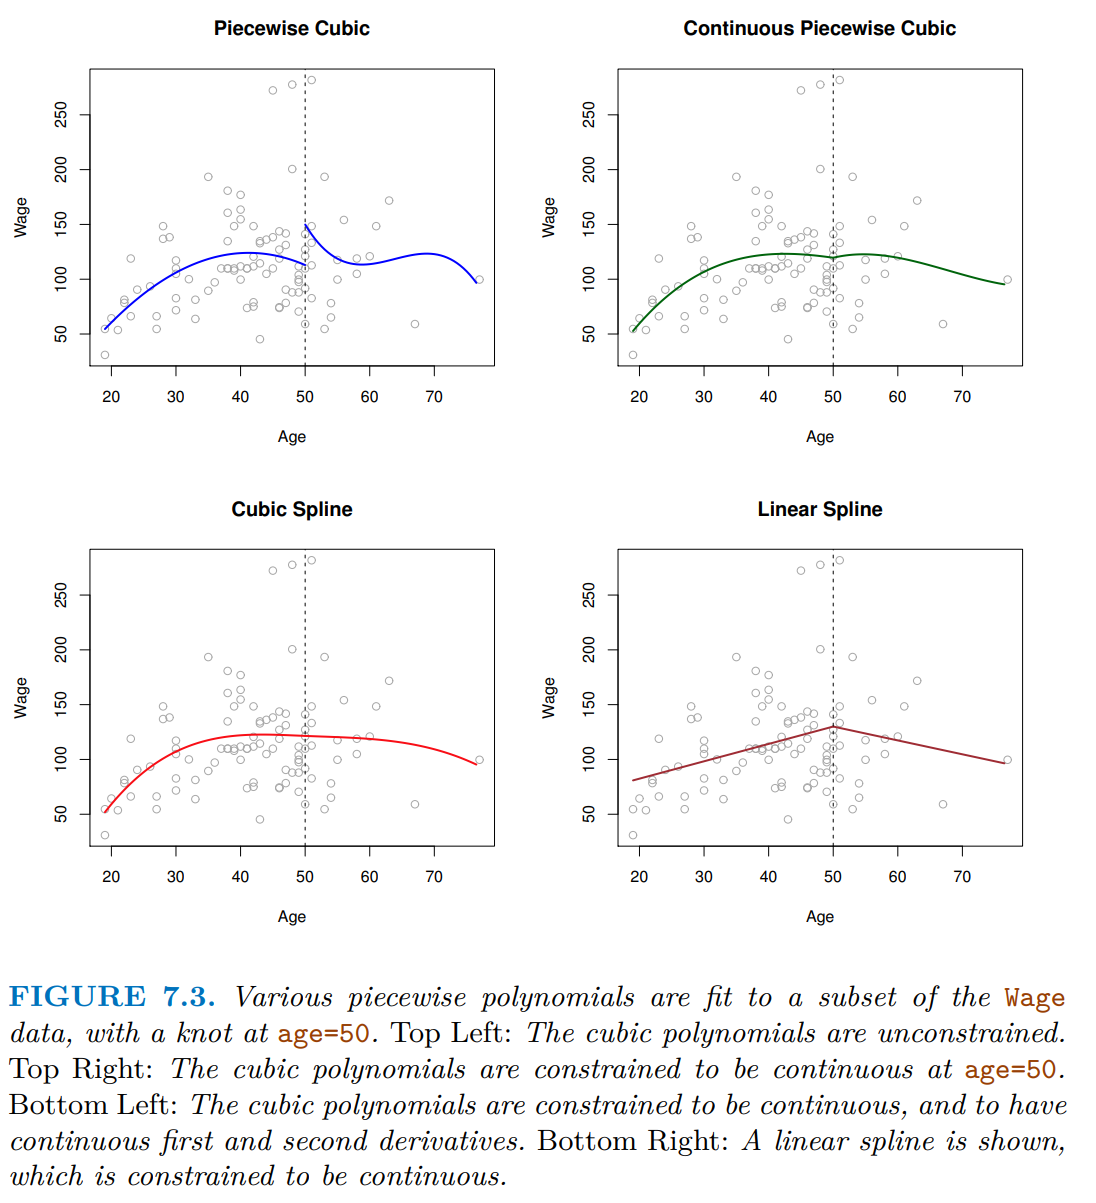
\includegraphics[width=0.8\textwidth]{Regression Splines Visualisations.png}
\end{center}

\subsubsection{Constraints and splines}
\begin{itemize}
    \item The fitted curve must be continuous
    \item The fitted curve should be very smooth
        \begin{itemize}
            \item For cubic spline: the first and second derivatives of the piecewise cubic function need to be continuous at each know
            \item For $d$-degree spline: the continuity in derivatives is required for up to degree $d-1$ at each knot
        \end{itemize}
    \item Each constraint we impose on the piecewise polynomials reduce on degree of freedom
    \item A \textit{natural spline} is a regression spline with linear boundary constraints: the spline function is required to be linear in the region where $X$ is the smaller than the smallest know, or larger than the largest knot
\end{itemize}

\subsubsection{Choosing the number and location of knots}
\begin{enumerate}
    \item Place more knots in places where we feel the function might vary most rapidly (place fewer knots where it seems more stable)
    \item Place knots in a uniform fashion. Firstly, specify the desired degrees of freedom, and then have software place the corresponding number of knots at uniform quantiles of the data.
\end{enumerate} \phantom{i}

\noindent \textbf{CV to choose optimal number of knots}
\begin{enumerate}
    \item Remove a portion of the data (e.g. $10\%$, then fit a spline with a certain number of knots to the remaining data
    \item Use fitted spline to make predictions for the held-out data
    \item Repeat steps 1-2 until each observation has been held-out once, and then compute the overall cross-validated RSS
    \item Repeat steps 1-3 for different number of knots $K$
    \item Value of $K$ that gives the smallest RSS is the optimal one
\end{enumerate} \phantom{i}

\noindent \textbf{Regression splines vs polynomial regression}
\begin{itemize}
    \item To increase flexibility, polynomial regression must use a high degree, while splines can simply increase number of knots but keeping the degree fixed. The latter generally produces more stable estimates
    \item Splines also allow us to adjust the position of the knots to create more flexibility. The polynomial regression doesn't have this feature
\end{itemize}

\subsection{Smoothing Splines}
\noindent Find some function $g(x)$ that can fit the observed data well. We need to consider both adherence and smoothness. \\

\noindent Adherence measured by the $RSS = \sum_{i=1}^{n}{(y_i - g(x_i))^2}$, and the smoothness can be measured by $\int g''(t)^2 \ dt$. Since there is a trade-off between adherence and smoothness, we construct the following objective function (with $\lambda \geq 0$): $\sum_{i=1}^{n}(y_i - g(x_i))^2 + \lambda \int g''(t)^2 \ dt$ (like \textit{loss} + \textit{penalty}). \\

\noindent \textbf{Some remarks:}
\begin{itemize}
    \item $\lambda = 0$: smoothness term has no effect. $g$ will be very jumpy and will exactly interpolate the training observations
    \item $\lambda \rightarrow \infty$, $g$ will be perfectly smooth
    \item So $\lambda$ controls the bias-variance trade-off of the smoothing spline
    \item Smoothing spline can be shown to be a nutral cubic spline with knots at the unique values of $x_1,...,x_n$
\end{itemize} \phantom{i}

\noindent \textbf{The effective degrees of freedom}:
\begin{itemize}
    \item $\lambda$ controls the smoothness of the spline, and hence hte effective degrees of freedom
    \item When $\lambda$ increases from $0$ to $\infty$, the effective degrees of freedom, denoted by $df_\lambda$, decrease from $n$ to $2$
    \item $df_\lambda$ is a measure of the flexibility of the smoothing spline
\end{itemize} \phantom{i}

\noindent \textbf{Choosing the smoothing parameter $\lambda$:} Find a value of $\lambda$ that makes the CV RSS as small as possible. LOOCV can also be computed for smoothing splines, using the following formula $RSS_{cv}(\lambda) = \sum_{i=1}^{n}{\Big[ \frac{y_i - \hat{g}_{\lambda}(x_i)}{1 - \{ \boldsymbol{S}_\lambda \}_{ii}} \Big]^2}$, where $\hat{\boldsymbol{g}}_\lambda = \boldsymbol{S}_{\lambda} \boldsymbol{y}$

\subsubsection{Smoothing splines in R}
\noindent A smoothing spline can be fit in R by \texttt{smooth.spline()} and one can specify \texttt{df} or $\lambda$ indirectly. \\

\noindent Example:
\begin{verbatim}
fit_ss <- smooth.spline(Wage$age, Wage$wage, df=16)
fit_ss2 <- smooth.spline(Wage$age, Wage$wage, cv=TRUE)
fit_ss2$df    # df selected by CV
\end{verbatim}
\noindent The second call chooses df by CV (checking many $\lambda$, picking that yields lowest CV error). Smoothing splines automatically choose many knots (at all data points) but with appropriate shrinkage, resulting in a smooth fit.

\subsection{Local Regression}
\noindent Local regression at $X = x_0$:
\begin{enumerate}
    \item Gather the fraction $s=\frac{k}{n}$ of training points whose $x_i$ are closest to $x_0$
    \item Assign a weight $K_{i0} = \omega \cdot \frac{x_i - x_0}{h(x_0)}$ to each point in this neighbourhood, where $h(x_0)$ is the bandwidth, the distance from $x_0$ to its $k$th closest $x_i$
    \item Fit a weighted least squares regression of the $y_i$ on the $x_i$ using the aforementioned weights, by finding $\hat\beta_0$ and $\hat\beta_1$ that minimise $\sum_{i=1}^{n}{K_{i0}(y_i - \beta_0 - \beta_1x_i)^2}$
    \item The fitted value at $x_0$ is given by $\hat{f}(x_0) = \hat\beta_0 + \hat\beta_1 x_0$
\end{enumerate} \phantom{i} \\
\noindent $s$ controls the flexibility of the non-linear fit. The smaller the $s$, the more local and wiggly will be our fit; alternatively, a very large $s$ will lead to a global fit to the data using all of the training observations. CV can be used to choose $s$. \\

\noindent \textbf{Why Local Regression?}
\begin{itemize}
    \item Adapts well to bias problems at boundaries and in regions of high curvature
    \item Easy to understand and interpret
    \item Methods have been developed that provide fast computation for one or more independent variables
    \item Very simple, can be used to work for different distributional assumptions
    \item A local model enables derivation of response adaptive methods for span value and polynomial order selection in a straightforward manner
\end{itemize} \phantom{i}

\noindent \textbf{How to choose polynomial degree?}: The choice is a bias-variance trade off. A higher degree will produce a less biased, but more variable estimate than a lower degree one. \\

\noindent \textbf{How to choose the weight function?} Want to consider a weight function $\omega(u)$ that are peaked at $u=0$ and that decay smoothly to $0$ as $u$ increases. A smooth weight function results in a smoother estimate. We also want a weight function that is nonzero only on a bounded interval, helping with computation speed.

\subsubsection{Local regression in R}
\noinednt In R, \texttt{loess()} or \texttt{ggplot2::geom\_smooth(method='loess')} can do this. Example:
\begin{verbatim}
fit_lo <- loess(wage ~ age, data=Wage, span=0.2)
\end{verbatim}

\subsection{Generalised Linear Models (GLMs)}
\begin{itemize}
    \item \textit{Probability distribution}: Instead of assuming normal distribution, GLMs work with distributions in the exponential family (e.g. normal, Poisson, binomial, and gamma)
    \item \textit{Model for the mean}: The mean is a linear function of hte predictors, $\boldsymbol{X}$, $E[Y] = f(\boldsymbol{X})$. In GLMs some smooth monotonic transformation of the mean is a linear function of $\boldsymbol{X}$. $g(E[Y]) = f(\boldsymbol{X})$.
\end{itemize} \phantom{i}

\noindent \textbf{Why GLMs:}
\begin{itemize}
    \item Easy to estimate standard errors, constructing CIs, testing, model selection and other statistical features
    \item GLMs are vary common in many areas of statistics, so they are constantly improving and we can draw upong developments from many industries
    \item There is standard software for fitting GLMs
    \item Although there is standard software companies create their own specialised GLMs so there is space to innovate
\end{itemize} \phantom{i}

\noindent \textbf{The exponential family and the link function:} \\
\noindent GLMs involve distributions that can be expressed in exponential form: $f(y|\theta, \phi) = e^{\frac{y\theta - b(\theta)}{\phi} + c(y,\theta)}$, $\theta$ is the canonical parameter, and $\phi$ is the dispersion parameter (that plays a role in defining the variance of $y$). \\

\noindent The canonical parameter $\theta$ is a function of $\mu$, denoted by $\theta(\mu)$, the canconical link function:
\begin{itemize}
    \item Normal: $\theta(\mu) = \mu$
    \item Poisson: $\theta(\mu) = \ln(\mu)$
    \item Exponential, gamma: $\theta(\mu) = -\mu^-1$
    \item Categorical, binomial, multinomial: $\theta(\mu) = \ln\Big( \frac{\mu}{1-\mu} \Big)$
\end{itemize}

\subsection{Generalised Additive Models (GAMs)}
\noindent GAMs extend multiple linear regression by allowing each variable to have its own non-linear effect, then adding them up:
$$y_i = \beta_0 + f_1(x_{i1}) + f_2(x_{i2}) + ... + f_p(x_{ip}) + \varepsilon_i$$
\noindent Could use and combine any non-linear methods such as local regression, polynomial regression, splines, or any combination of the approaches discussed. Also could use qualitative variables using dummy variables.
\subsubsection{Pros and Cons}
\noindent \textbf{Pros}
\begin{itemize}
    \item GAM allow non-linear $f_j$ to each $X_j$ and does it automatically, so we don't need to manually try out many different transformations.
    \item Non-linear fit could make more accurate predictions.
    \item Since model is additive, we can still examine the effect of each $X_j$ on $Y$ individually while holding all the other variables fixed. Hence GAMs provid useful inference.
    \item Smoothness of function $f_j$ for $X_j$ can be summarised via degrees of freedom.
\end{itemize} \phantom{i}

\noindent \textbf{Cons}
\begin{itemize}
    \item Restricted to be additive. Imporatnt interactions may be missed, however we can add interaction terms to the GAM model by including additional predictors of the form $X_j \times X_k$. In addition we can add low-dimensional interaction functions of the form $f_{jk}(X_j, X_k)$; such terms can be fit using two-dimensional smoothers such as local regression.
\end{itemize}

\subsubsection{GAMs in R}
\noindent For example, a GAM might be:
\[ \widehat{\text{wage}} = \beta_0 + f_1(\text{year}) + f_2(\text{age}) + f_3(\text{education}), \]
with $f_1, f_2$ as splines and $f_3$ as a factor effect (education is qualitative with categories, which GAM handles as dummy functions). \\

\noindent In R, using package \texttt{gam} (or \texttt{mgcv} for a more modern approach):
\begin{verbatim}
library(gam)
gam_fit <- gam(wage ~ s(year, 4) + s(age, 5) + education, data=Wage)
summary(gam_fit)
plot(gam_fit, se=TRUE, col="blue")
\end{verbatim}
\noindent Here \texttt{s(year,4)} uses a smoothing spline or basis with df=4 for year, \texttt{s(age,5)} uses df=5 for age. The \texttt{plot} function will show the estimated $f_1(\text{year})$ and $f_2(\text{age})$ curves with confidence bands. The summary can give approximate significance of each $f_j$ (via an $F$ test comparing to a flat function).

\section{Logistic Regression and Bayes Theorem}

However, the key new topic in Week 6 was \textbf{Logistic Regression}, a classification method.

\subsection{Classification Methods (Introduction)}
Types:
\begin{enumerate}
    \item Logistic regression
    \item Linear discriminant analysis (LDA)
    \item Quadratic discriminant analysis (QDA)
    \item Naive Bayes
    \item K-nearest neighbours
    \item Classification trees
    \item Support vector machines
\end{enumerate}
\vspace{1em} \noindent Used to capture a qualitative variable instead of a quantitative one. Why can't we encode a variable using linear regression past a binary response? (a) A regression method cannot accommodate a qualitative response with more than two classes (as order of the classes matters and how different they are to each other matters in regression), (b) A regression method will not provide meaningful estimates of $Pr(Y|X)$, even with just two classes.


\subsection{Logistic Regression Theory}
For a binary outcome $Y$ (two classes, often coded as 0/1 for convenience), logistic regression models the \textbf{probability} of $Y=1$ as a function of predictors $X$. We write:
\[ p(X) = P(Y=1 \mid X) = \frac{\exp(\beta_0 + \beta_1 X_1 + \cdots + \beta_p X_p)}{1 + \exp(\beta_0 + \beta_1 X_1 + \cdots + \beta_p X_p)}. \]
This is the \textbf{logistic function} mapping $\mathbb{R}$ to $(0,1)$. It ensures predicted probabilities stay between 0 and 1, unlike a linear model. \\

\noindent The logistic model: $p(X) = \frac{e^{\beta_{0}  + \beta_{1}X}}{1 + e^{\beta_{0} + \beta_{1}X}}$ and the multiple logistic regression: $p(\boldsymbol{X}) = \frac{e^{\beta_{0} + \beta_{1}X_{1} + ... + \beta_{p}X_{p}}}{1 + e^{\beta_{0} + \beta_{1}X_{1} + ... + \beta_{p}X_{p}}}$ \\

\noindent Taking odds:
\[ \frac{p(X)}{1-p(X)} = \exp(\beta_0 + \beta_1 X_1 + \cdots + \beta_p X_p) \in (0, \infty), \]
If odds close to $0 \implies $ very low probability of $X$ and odds close to $\infty \implies$ very high probability of $X$. \\
\noindent So the \textbf{log-odds} (logit) is linear:
\[ \log\frac{p(X)}{1-p(X)} = \beta_0 + \beta_1 X_1 + \cdots + \beta_p X_p. \]

\noindent Interpretation: $\beta_j$ now is the change in log-odds for a one unit increase in $X_j$, holding others fixed. Equivalently, $e^{\beta_j}$ is the multiplicative change in the odds for a one-unit increase in $X_j$. For example, if $\beta_j = 0.7$, then odds are $e^{0.7}\approx2.01$ times greater for a one-unit increase in $X_j$ (meaning $p$ roughly doubles, if in mid-range).

\noindent Logistic regression is fit by \textbf{maximum likelihood} rather than least squares (since it's not a linear model in $Y$). The likelihood for independent observations is 
\[ L(\beta_0,\boldsymbol{\beta}) = \prod_{i: y_i=1} p(x_i) \prod_{j: y_j=0} [1-p(x_j)], \]
and we find $\hat\beta$ that maximize this (often via iterative algorithms).  \\

\noindent The output in R often includes:
\begin{itemize}
    \item Coefficients (values of $\beta_j$), measures relationship of each predictor with the response
    \item Standard error (SE$(\beta_j)$)
    \item $z$-statistics ($\frac{\hat{\beta}_j}{\text{SE}(\hat{\beta}_j)}$)
    \begin{itemize}
        \item A large (absolute) value of the $z$-statistic indicates evidence against the null hypothesis $H_0: \; B_j = 0$ (meaning there is a meaningful relationship between the predictor $X_j$ and $Y$)
    \end{itemize}
    \item P-values. If $p$ is tiny, we can reject $H_0 \implies$ there is a meaningful relationship between $X_j$ and $Y$
\end{itemize} 
\phantom{i}
\\ \noindent We measure model fit by \textbf{deviance} or by classification performance metrics, since $R^2$ isn't meaningful here. One can compute a pseudo-$R^2$ or just measure accuracy. \\

\noindent \textbf{Prediction rule:} To make a classification, we predict class 1 if $\hat p(X) > 0.5$ (or another cutoff). 0.5 is the default threshold for equal costs. Sometimes we adjust the threshold for specific sensitivity or specificity needs (e.g., predict positive if probability $>$ 0.2 to catch more positives at cost of more false alarms, as shown by altering threshold in slides for LDA; similar logic applies to logistic). \\

\noindent \textbf{Making predictions:} Once you have coefficients, we can compute the probability of event $X$ (use probability of default as the example). E.g. if credit card balance $X = \$1,000$, $\hat{p}(X) = \frac{e^{\hat{\beta}_{0} + \hat{\beta}_{1}X}}{1 + e^{\hat{\beta}_{0} + \hat{\beta}_{1}X}} = \frac{e^{-10.6513 + 0.0055 \times 1000}}{1 + e^{-10.6513 + 0.0055 \times 1000}} = 0.00576$ \\

\noindent \textbf{Qualitative predictors (dummy variable encoding):} Can fit a model and the predictor can be $0$ if some condition is satisfied, and $1$ if not, then can fit a simple logistic model based on that. \\

\noindent \textbf{Pros:}
\begin{itemize}
    \item  Outputs probabilities, which is more informative than just class labels (especially in insurance, you might use the probabilities for decision).
    \item Well-calibrated (if model is correct, predicted probabilities tend to reflect true frequencies).
    \item Inference is available (Wald tests via $z$-values).
    \item Can naturally extend to multiple classes (via multinomial logistic, not covered deeply but concept exists).
\end{itemize}


\noindent \textbf{Cons:}
\begin{itemize}
    \item Assumes a linear log-odds relationship. If the true decision boundary is highly non-linear, logistic (without polynomial terms or interactions) will mis-specify.
    \item It’s parametric; if parametric form is wrong, could be biased.
    \item In practice, if classes are not well separated, parameter estimates have large uncertainty (though still optimal in max likelihood sense).
\end{itemize}

\subsection{Logistic Regression in R (Example: Smarket Data)}
The \texttt{Smarket} dataset (from \texttt{ISLR}) has daily stock market direction data. We'll use logistic regression to predict \texttt{Direction} (Up/Down) based on lagged returns.

\begin{verbatim}
library(ISLR)
?Smarket   # info on dataset
glm_fit <- glm(Direction ~ Lag1 + Lag2 + Lag3 + Lag4 + Lag5 + Volume,
               data = Smarket, family = binomial)
summary(glm_fit)
\end{verbatim}
We use \texttt{glm(..., family=binomial)} for logistic regression. The summary might show:
\begin{verbatim}
Coefficients:
             Estimate Std. Error z value Pr(>|z|)
(Intercept)  -0.1260   0.240    -0.525   0.600
Lag1         -0.0731   0.051    -1.430   0.152
Lag2         -0.0423   0.051    -0.830   0.407
Lag3          0.0111   0.051     0.218   0.827
Lag4          0.0094   0.051     0.184   0.854
Lag5          0.0103   0.051     0.202   0.840
Volume       -0.1350   0.158    -0.855   0.392
\end{verbatim}
None of the lags are significant (high p-values), meaning no strong linear relationship to today's market direction. (This is a known result: logistic regression can't predict much here.)

We can compute predicted probabilities of market going Up:
\begin{verbatim}
glm_probs <- predict(glm_fit, type="response")  # on training data
glm_probs[1:5]
# For classification, use threshold 0.5:
glm_pred <- ifelse(glm_probs > 0.5, "Up", "Down")
table(glm_pred, Smarket$Direction)
\end{verbatim}
The table might show something like: model predicts Up all days (common if probabilities ~0.5). Indeed, logistic might give around 0.5 for all since no significant predictors.

We then realize we should try a different approach: perhaps use only Lag1 and Lag2 as predictors (since others clearly not helpful) and test on 2005 data (held out). In lab, they did:
\begin{verbatim}
train <- (Year < 2005)
Smarket.2005 <- Smarket[!train, ]
glm_fit2 <- glm(Direction ~ Lag1 + Lag2, data=Smarket, family=binomial, subset=train)
glm_probs2 <- predict(glm_fit2, Smarket.2005, type="response")
glm_pred2 <- ifelse(glm_probs2 > 0.5, "Up", "Down")
table(glm_pred2, Smarket.2005$Direction)
mean(glm_pred2 == Smarket.2005$Direction)
\end{verbatim}
This yields a confusion matrix and accuracy on test set (2005). Perhaps ~56\% accuracy, better than random 50\% and better than using all lag variables which gave ~50\% hit rate.

The confusion matrix allows computing \textbf{sensitivity} (true positive rate) and \textbf{specificity} (true negative rate). For example, if "Up" is positive class: sensitivity = correctly predicted Ups / total actual Ups; specificity = correctly predicted Downs / total actual Downs. By changing the threshold (like 0.5 to 0.3), one can increase sensitivity at cost of specificity.

\textbf{Important formulas:} 
- For one predictor, logistic has $p(X) = \frac{e^{\beta_0+\beta_1 X}}{1+e^{\beta_0+\beta_1 X}}$. We often talk about \textbf{odds ratio}: $e^{\beta_1}$ is the odds ratio for a unit change in $X$. 
- For model inference, $z = \frac{\hat\beta_j}{\text{SE}(\hat\beta_j)}$ approximately $\sim N(0,1)$ under $H_0$.
- Null deviance and residual deviance can be used like SSR and SSE analogies for significance of full model (Chi-square test comparing to null model). \\

\noindent \textbf{Pros/Cons Recap:} Logistic regression is a fundamental classification approach and works well when class separation is linear in log-odds. It's interpretable (odds ratios). But if decision boundary is more complex, we need other methods (Week 7 onward covers LDA/QDA, KNN, etc., which are alternatives). \\

\subsection{Bayes' theorem for classification:}
\noindent Suppose we wish to classify an observation into one of $K$ classes ($K \geq 2$). \\

\noindent Let $\pi_{k}$ denote the overall or \textit{prior} probability that a randomly chosen observation comes from class $k$. \\

\noindent Let $f_k(x) = \mathbb{P}(X=x|Y=k)$ be the density function of $X$ for an observation that comes from the $k$th class:
\begin{itemize}
    \item $f_k(x)$ is relatively large if there is a high prob. that an observation in the $k$th class $X \approx x$;
    \item $f_k(x)$ is relatively small if it is unlikely that an observation in the $k$th class has $X \approx x$.
\end{itemize}
\phantom{i}
\\ \noindent Then Bayes' theorem states that:
$$p_k(x) = \mathbb{P}(Y=k|X=x) = \frac{\pi_k f_k(x)}{\sum_{I=1}^{K}{\pi_I f_I(x)}}$$
\noindent We can estimate $\pi_k$ and $f_k(x)$ seperately and then plug in those estimatees into the equation above to obtain an estimate of $p_k(x)$. \textit{LDA}, \textit{QDA} and \textit{naive Bayes} all use different estimates of $f_k(x)$.

\section{Linear/Quadratic Discriminant Analysis and KNN}
\subsection{LDA Theory}

\subsubsection{LDA for $p = 1$:}
\noindent We only have $1$ predictor, $f_k(x) = \frac{1}{\sqrt{2\pi}\sigma_{k}}e^{-\frac{(x-\mu_k)^2}{2\sigma_{k}^{2}}}$, assume that $\sigma_1^2 = ... = \sigma_k^2 = \sigma^2$. Therefore:

$$p_k(x) = \frac{\pi_k e^{-\frac{(x - \mu_k)^2}{2\sigma^2}}}{\sum_{I=1}^{K}{\pi_I  e^{-\frac{(x - \mu_k)^2}{2\sigma^2}}}}$$

\noindent \textbf{How to classify an observation $\boldsymbol{X = x}$}: We take $\delta_k(x) = \ln(p_k(x))$ and try to maximise it. Re-arrange terms to get $\delta_k(x) = x \cdot \frac{\mu_k}{\sigma^2} - \frac{\mu_k^2}{2\sigma^2} + \log(\pi_k)$. \\

\noindent E.g. If $K=2$ and $\pi_1 = 0.5$. Find the condition that $x$ needs to satisfy such that the Bayes classifier assigns observation $X=x$ to class $1$: \\

\begin{align*}
    \text{For } & \mu_1 > \mu_2: \\
    \delta_1(x) > \delta_{2}(x) &\Leftrightarrow x(\mu_1 - \mu_2) - \frac{1}{2}(\mu_1^2 - \mu_2^2) > 0 \\
    &\Leftrightarrow x > \frac{\mu_1 + \mu_2}{2} \Leftrightarrow Y = 1
\end{align*}

\noindent Clearly, if $\mu_1 < \mu_2$, then $x < \frac{\mu_1 + \mu_2}{2}$. The point $x = \frac{\mu_1 + \mu_2}{2}$ is the Bayes decision boundary. \\

\noindent \textbf{Estimations used in LDA:} LDA estimates parameters then plugs them into $\delta_k(x)$. Assume $n$ is the total \#observations in the training data set, and $n_k$ is the number of training observations in the $k$th class. \\

\begin{align*}
    \hat{\mu}_k &= \frac{1}{n_k} \sum_{i: y_i = k}{x_k} \\
    \hat{\sigma}^2 &= \frac{1}{n-K}\sum_{k=1}^{K}\sum_{i: y_i = k}(x_i - \hat{\mu_k})^2 \\
    \hat{\pi}_k &= \frac{n_k}{n} \\
    \implies \hat{\delta}_k(x) &= x \cdot \frac{\hat{\mu}_k}{\hat{\sigma}^2} - \frac{\hat{\mu}_k^2}{2\hat{\sigma}^2} + \log(\hat{\pi}_k), \ \text{linear discriminant function of $x$}
\end{align*}

\noindent \textit{The LDA classifier results from assuming that the observations within each class come from a normal distribution with a class-specific mean vector and common variance $\sigma^2$}.

\subsubsection{LDA for $p > 1$:}
\noindent We have $p$-predictors, let $\boldsymbol{X} \sim N(\boldsymbol{\mu}, \boldsymbol{\Sigma})$, Cov($\boldsymbol{X}$) = $\boldsymbol{\Sigma}$, $\implies$ the pdf:
$$f(\boldsymbol{x}) = \frac{1}{(2\pi)^{p/2}\sqrt{|\boldsymbol{\Sigma}|}}e^{-\frac{1}{2}(\boldsymbol{x} - \boldsymbol{\mu})\boldsymbol{\Sigma}^2(\boldsymbol{x} - \boldsymbol{\mu})^\top}$$
$$\delta_k(\boldsymbol{x}) = \boldsymbol{x}\boldsymbol{\Sigma}^{-1}\boldsymbol{\mu}_k^\top - \frac{1}{2}\boldsymbol{\mu}_k^{\top} + \log(\pi_k)$$

\noindent Then we can estimate the unknown parameters like before, to classify a new observation $\boldsymbol{X} = \boldsymbol{x}$, LDA plugs these estimates into $\delta_k(\boldsymbol{x})$ and classifies to the class with the largest $\delta_k(\boldsymbol{x})$. \\

\noindent \textbf{A binary classification problem example:} $10,000$ observations in \textit{Default} training data set, where $333$ individuals defaulted. Perform LDA on the training data and the training error rate is $2.75\%$, some remarks:
\begin{itemize}
    \item The training error rate being low doesn't mean the test error will be low as well, over fitting is a potential issue, in particular when $p$ is close to $n$.
    \item Since only $3.33\%$ of individuals in training data defaulted, the \textit{null} classifier, which always predicts no defaulting, will achieve an training error rate of $3.33\%$, not much higher than the LDA training error rate.
    \item  What does the credit card company really care about?
\end{itemize}
\phantom{i} \\
\noindent Confusion matrix:
\begin{center}
  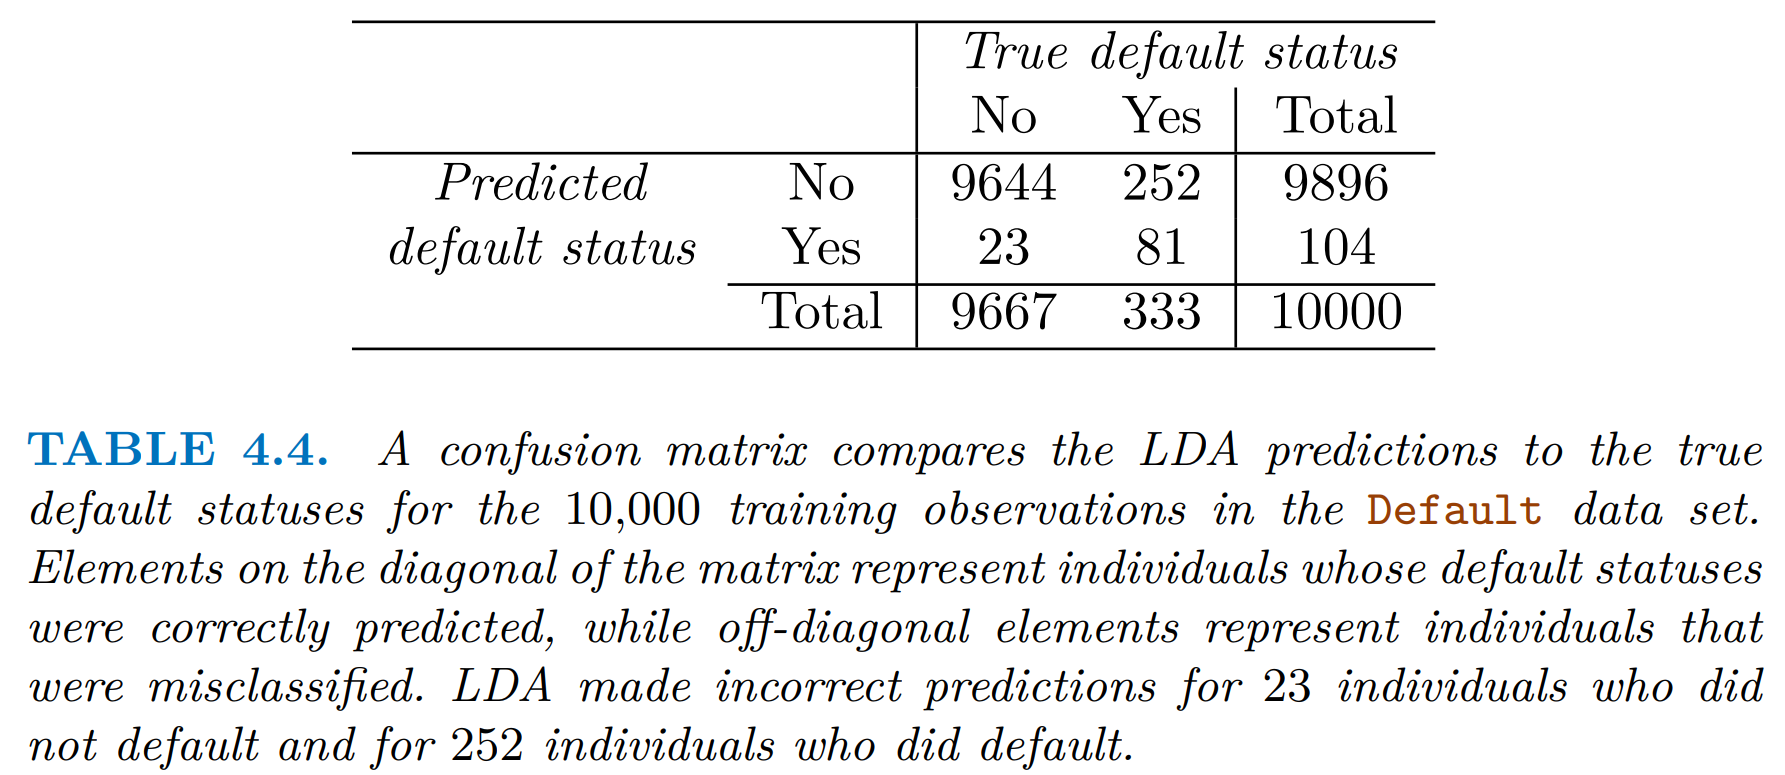
\includegraphics[width=0.8\textwidth]{LDA Example Confusion Matrix.png}
\end{center}

\begin{itemize}
    \item Training error rate is $(252+23)/10000 = 2.75\%$.
    \item Assigning not defaulted individuals to \textit{default} error: $23/9667 = 0.24\%$.
    \item Assigning defaulted individuals to \textit{no default} error: $252/333 = 75.7\%$.
\end{itemize}
\phantom{i} \\
\noindent Is the LDA classifier a satisfactory one?
\begin{itemize}
    \item \textit{Sensitivity} of the LDA classifier: $81/333 = 24.3\%$; very poor!
    \item \textit{Specificity} of the LDA classifer: $9664/9667 = 99.8\%$; Great!
    \item Poor sensitivity so not a satisfactory classifier, since credit card company would usually care more about not incorrectly classifying an individual who will default as no default.
\end{itemize}
\phantom{i} \\
\noindent Can we modify the LDA to better meet the credit card company's need?
\begin{itemize}
    \item Yes. We can modify the threshold used in the LDA approach to achieve the goal. The default threshold is $0.5$, i.e. we assign an observation to the \textit{default} class if $\mathbb{P}(\text{default} = \text{Yes}|\boldsymbol{X} = \boldsymbol{x}) > 0.5$.
    \item If threshold is now $20\%$ sensitivity is better, specificity is still great which is really good although the overall error rate increases a little bit.
\end{itemize}
\phantom{i} \\
\noindent \textbf{Threshold vs. Error Rate Curve:}
\begin{center}
  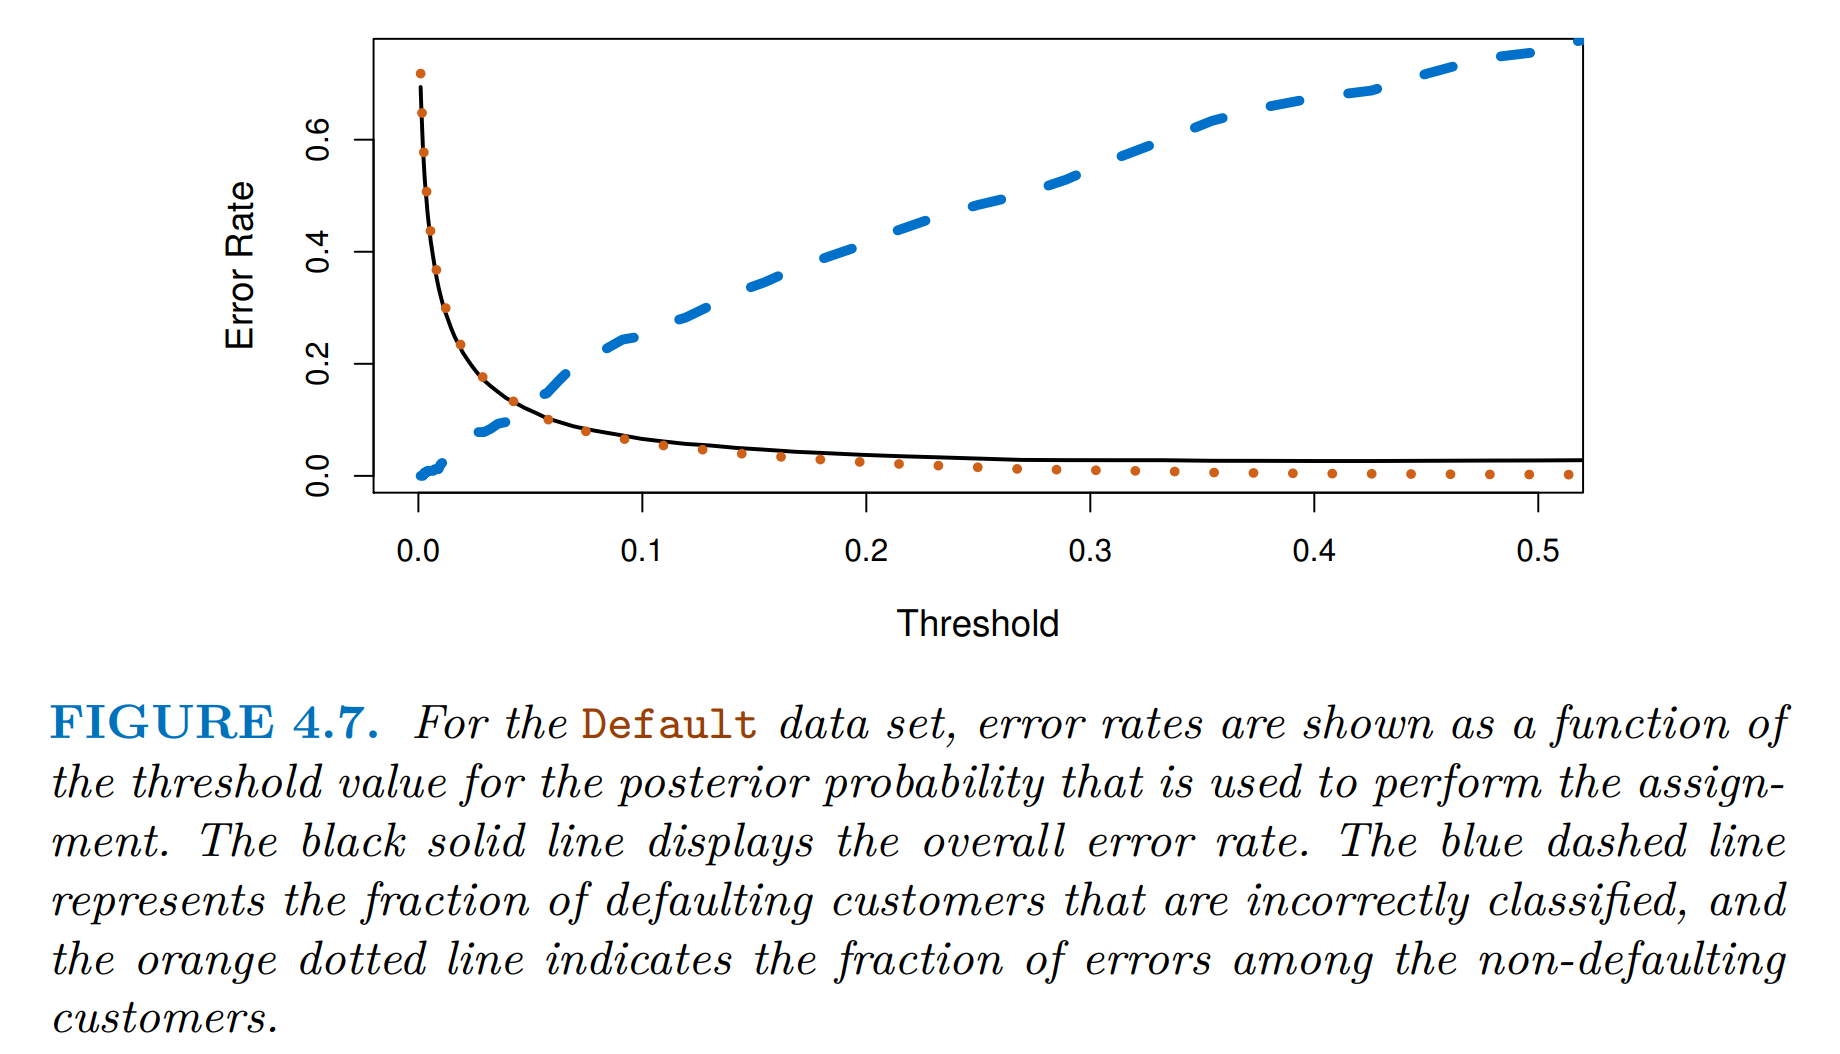
\includegraphics[width=0.8\textwidth]{LDA Example Threshold vs Error Rate.png}
\end{center}
\vspace{7em}
\noindent \textbf{ROC (Receiver Operating Characteristics) Curve:} \\
\noindent How to read: the overall performance of a classifier, summarised over all possible thresholds, is given by the \textit{area under the (ROC) curve} (AUC). An ideal ROC curve will hug the top left corner, so the larger the AUC the better the classifier.
\begin{center}
  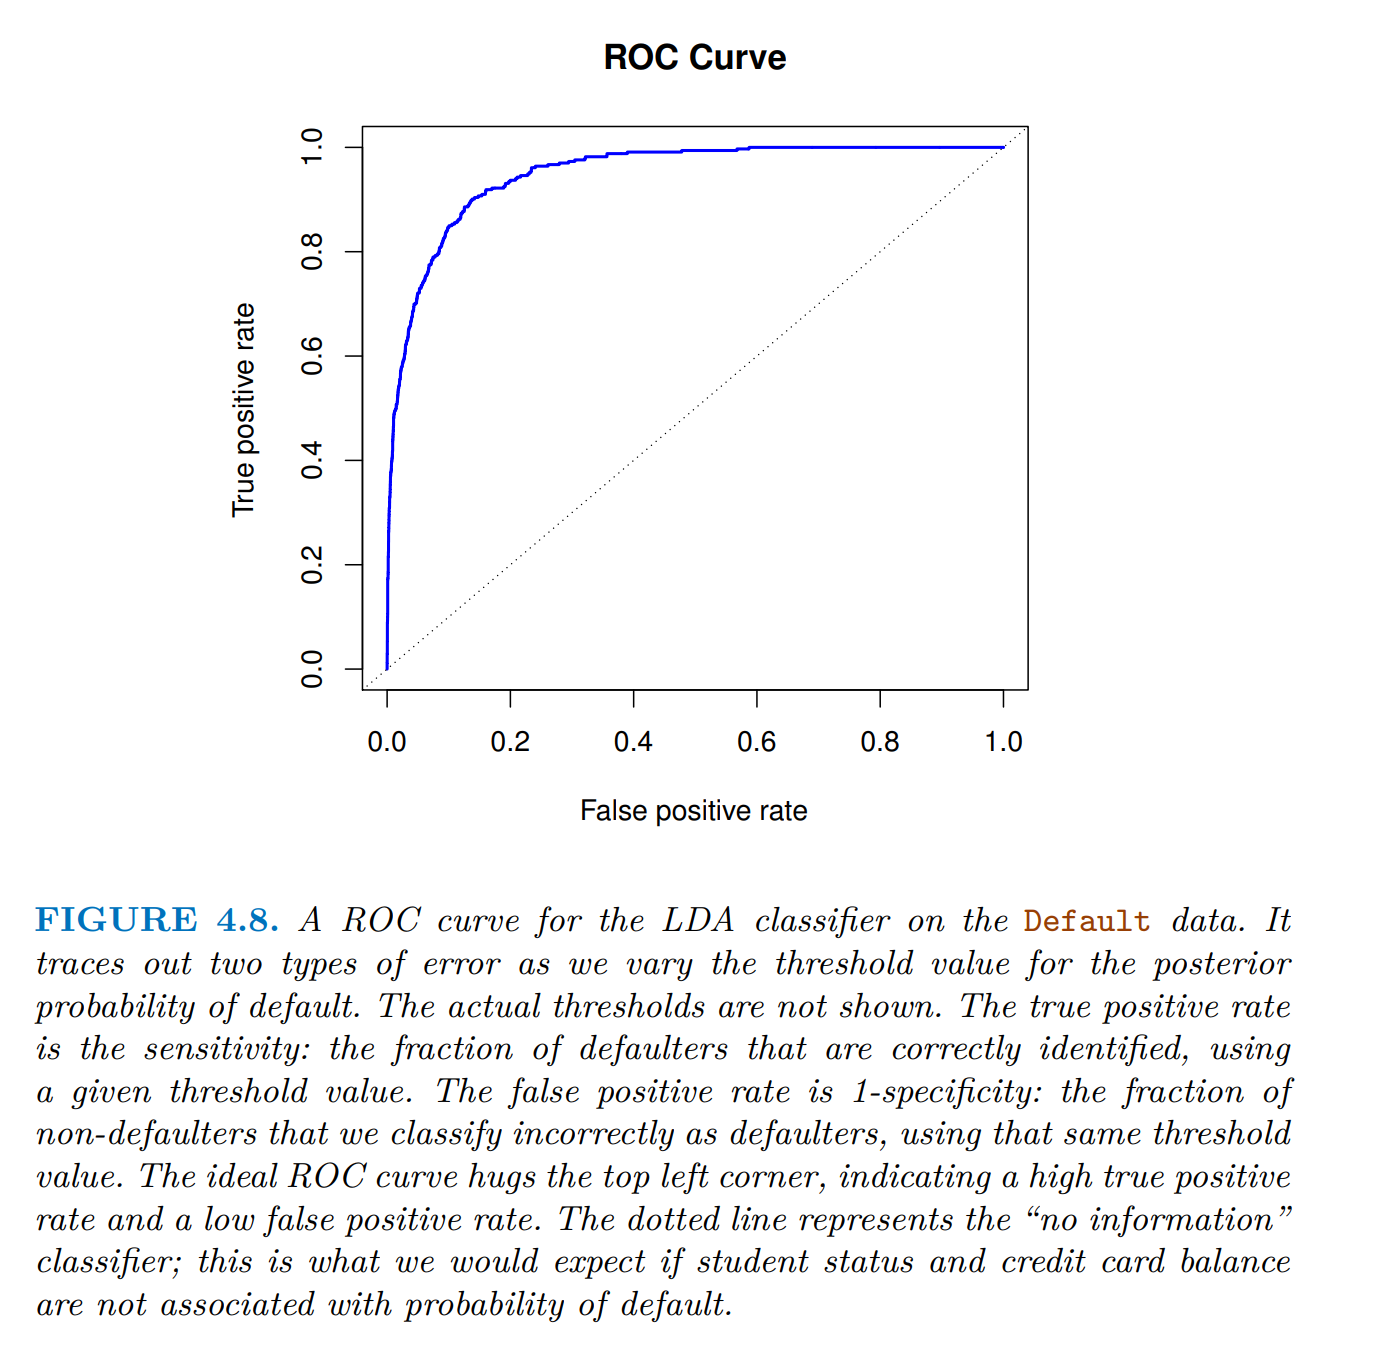
\includegraphics[width=0.8\textwidth]{LDA Example ROC Curve.png}
\end{center}
\phantom{i}\\

\subsection{Confusion Matrices and Measures for Classification}

\begin{center}
  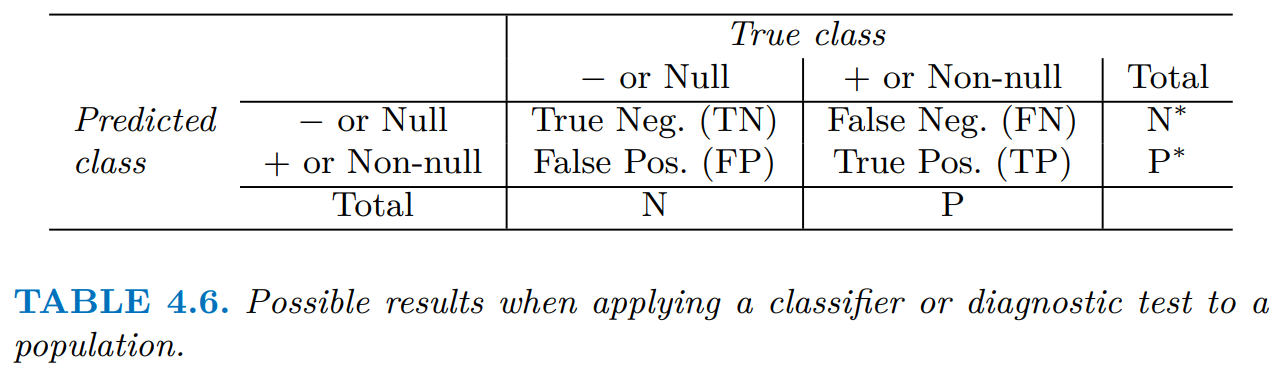
\includegraphics[width=0.8\textwidth]{Classificaiton Confusion Matrix Definition.png}
\end{center}

\begin{center}
  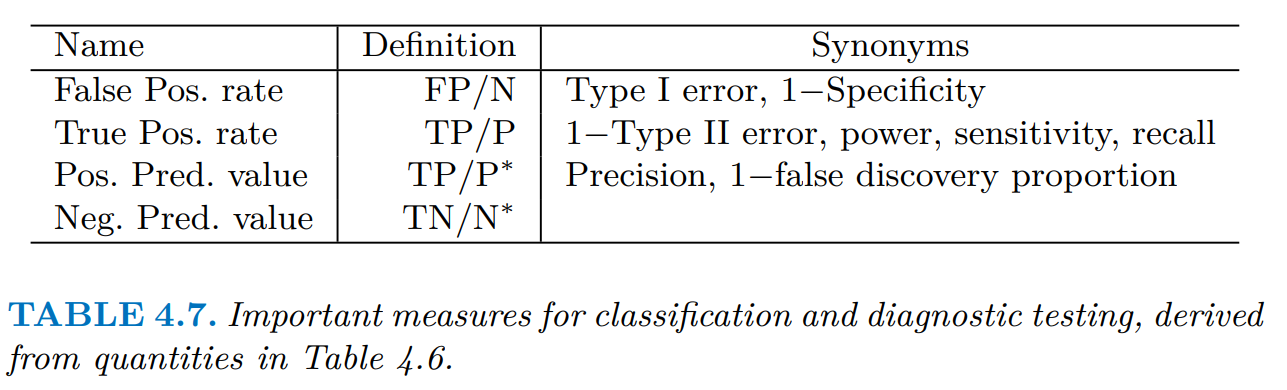
\includegraphics[width=0.8\textwidth]{Measures of Classification.png}
\end{center}

\subsubsection{Confusion Matrices in R}
\begin{verbatim}
table(predictions, response variable)
mean(predictions == response variable) # true positive rate
\end{verbatim}

\subsection{Quadratic Discriminant Analysis (QDA):}
Assumes that an observation from the $k$th class is one of the form $\boldsymbol{X} \sim N(\boldsymbol{\mu}_k, \boldsymbol{\Sigma}_k)$, so unique covariance matrices for each class. Therefore we can derive:
\begin{align*}
    \delta_{x}(\boldsymbol{x}) &= -\frac{1}{2}(\boldsymbol{x} - \boldsymbol{\mu}_k)\boldsymbol{\Sigma}_{k}^{-1}(\boldsymbol{x - \boldsymbol{\mu}_k})^\top - \frac{1}{2}\log|\boldsymbol{\Sigma}_k| + \log(\pi_k) \\
    &= -\frac{1}{2}\boldsymbol{x}\boldsymbol{\Sigma}_k^{-1}\boldsymbol{x}^\top + \boldsymbol{x}\boldsymbol{\Sigma}_{k}^{-1}\boldsymbol{\mu}_{k}^{\top} - \frac{1}{2}\boldsymbol{\mu}_k\boldsymbol{\Sigma}_k^{-1}\boldsymbol{\mu}_k^{\top} - \frac{1}{2}\log|\boldsymbol{\Sigma}_k| + \log(\pi_k)
\end{align*}

\noindent Then we plug in estimates for $\boldsymbol{\Sigma}_k$ and $\boldsymbol{\mu}_k$ to assign an observation to the class for which this quantity is the largest, $\boldsymbol{x}$ appears as a quadratic function in the equation above so that's why its a QDA.

\subsubsection{When to use QDA or LDA?}
\noindent The answer depends on the bias-variance trade-off:
\begin{itemize}
    \item LDA is much less flexible classifier than QDA, which lead to lower variance. Since, for $p$ predictors, QDA estimates $K\frac{p(p+1)}{2}$ params. and LDA estaimtes $\frac{p(p+1)}{2}$ params.
    \item If LDA's assumption on common covariance matrix is not appropriate, then it will result in higher bias
    \item LDA tends to be a better bet than QDA if there are relatively fewer training observations and so reducing variance is crucial.
    \item QDA is recommended if the training set is very large, or if the assumption of common covariance matrix for the $K$ classes is clearly untenable (not that great).
\end{itemize}



\subsection{LDA in R (Example: Smarket Data continued)}
We apply LDA to the Smarket data (Years <2005 as training, 2005 as test) to compare with logistic:
\begin{verbatim}
library(MASS)
lda_fit <- lda(Direction ~ Lag1 + Lag2, data=Smarket, subset=Year<2005)
lda_fit
\end{verbatim}
The output shows the means for the two classes for Lag1 and Lag2, and the common covariance (in terms of scaling factors). For example, it may output:
\begin{verbatim}
Mean for Down: Lag1=0.042, Lag2=0.033
Mean for Up:   Lag1=-0.039, Lag2=-0.031
\end{verbatim}
And perhaps prior probabilities (approx 0.5/0.5 if balanced data).

To predict:
\begin{verbatim}
lda_pred <- predict(lda_fit, Smarket.2005)
names(lda_pred)
# lda_pred is a list with components: class (predicted class labels),
# posterior (probabilities for each class), x (discriminant scores)
head(lda_pred$posterior)
head(lda_pred$class)
\end{verbatim}
We then compute confusion matrix:
\begin{verbatim}
table(lda_pred$class, Smarket.2005$Direction)
mean(lda_pred$class == Smarket.2005$Direction)
\end{verbatim}
The performance might be similar or slightly different from logistic (with these two predictors, likely similar ~56% accuracy).

If we want to use a threshold different from 0.5, we can manually check posterior probabilities. For instance, to get more "Up" predictions, lower threshold:
\begin{verbatim}
lda_highThreshold <- ifelse(lda_pred$posterior[,"Up"] > 0.55, "Up", "Down")
\end{verbatim}
and then check sensitivity etc. Typically with equal priors and costs, threshold=0.5 is default. But if say false negatives are worse, you'd pick a lower threshold to catch more positives.

\textbf{Interpretation:} LDA finds a linear combination of Lag1 and Lag2 that separates \texttt{Up} vs \texttt{Down}. We could examine \texttt{lda\_pred\$x\$}, which is the discriminant value $x^\top \hat{\Sigma}^{-1}(\hat{\mu}_{\text{Up}} - \hat{\mu}_{\text{Down}})$ (one dimension because two classes yield one discriminant axis). We could see how a cutoff on that corresponds to the classification boundary.

\subsection{LDA/QDA in R (Example: Weekly Data or Simulated)}
Using the \texttt{Smarket} example above, QDA is just:
\begin{verbatim}
qda_fit <- qda(Direction ~ Lag1 + Lag2, data=Smarket, subset=Year<2005)
qda_fit
qda_pred <- predict(qda_fit, Smarket.2005)$class
table(qda_pred, Smarket.2005$Direction)
mean(qda_pred == Smarket.2005$Direction)
\end{verbatim}
In that particular data, QDA might perform similarly or a tad worse if there isn’t a strong quadratic difference (the text noted QDA got about 0.599 accuracy on Smarket vs LDA 0.56, meaning here QDA did slightly better, possibly fluke given small improvement).

But generally one would try LDA first, and if evidence suggests need for QDA (maybe significant quadratic terms in logistic, or separate class variances), then QDA.

We also introduced \textbf{comparison of classifiers}:
- One can compare error rates.
- Or use \textbf{ROC curves} (Receiver Operating Characteristic) which plot sensitivity vs 1-specificity as threshold varies. The area under ROC (AUC) is a threshold-independent measure of classifier performance.

We might not have deeply covered ROC in lecture 7, but it was in lab code for SVM. But logically belongs to classification evaluation. Perhaps they introduced it conceptually in classification.

Finally, week 7 introduced another classifier: \textbf{K-Nearest Neighbors (KNN)}.

\subsection{K-Nearest Neighbors (KNN) Theory}
KNN is a non-parametric classification method:
To predict class for an observation $x_0$, find the $K$ training observations closest to $x_0$ (in Euclidean distance, typically). Then have them vote (majority class among those $K$ neighbors). The estimated probability for class $j$ is the fraction of the $K$ neighbors that belong to class $j$:
\[ \Pr(Y=j|X=x_0) = \frac{1}{K} \sum_{i \in N_0} I(y_i = j), \] 
where $N_0$ is the index set of the $K$ nearest neighbors of $x_0$. Then assign the class with highest estimated probability.

\subsubsection{Choosing a K Value}
\begin{itemize}
    \item KNN is very flexible: as $K \to n$, it becomes very smooth (predict majority of entire training set = always most frequent class, high bias, low variance).
    \item As $K \to 1$, it can get very wiggly (each point is basically its own neighborhood, can overfit noise, low bias, high variance).
    \item We choose $K$ by cross-validation typically.
\end{itemize}

\subsubsection{Pros an cons of KNN approach}
\begin{itemize}
    \item \textbf{Pros:}
        \begin{enumerate}
            \item The algorithm is simple and easy to implement.
            \item There is no need to build a model, tune several parameters, or make additional assumptions (like shape of decision boundary).
            \item The algorithm is versatile. It can be used for classification and regression.
            \item Effective if $n$ is very large (lots of data) and relationship is hard to parametric form.
        \end{enumerate}
    \item \textbf{Cons:}
        \begin{enumerate}
            \item No explicit model, so no interpretability beyond "these neighbors vote".
            \item Doesn’t give confidence intervals or the like, though one can derive some asymptotic analysis if needed.
            \item Slow if $n$ is large (need to compute distances to all points for each prediction, though can use indexing structures to speed up).
            \item Curse of dimensionality. KNN works poorly if $p$ is large, because distance in high dimension becomes less meaningful (all points become far). Requires feature scaling or selection and often needs a lot of data.
        \end{enumerate}
\end{itemize}

\subsection{Comparison of Logistic regression and LDA}
\noindent Both methods produce a linear decision boundary, the only difference between the two approaches is that $\beta_0$ and $\beta_1$ are estimated by MLE, whereas $c_0$ and $c_1$ are computed using the estaimtes mean and variance from a normal distribution (also holds for $p > 1$). \\

\noindent Proof: logistic regression $\log(\frac{p_1(x)}{1-p_{1}(x)}) = \beta_0 + \beta_1 x$ and LDA $\log(\frac{p_1(x)}{1-p_1(x)}) = \log(\frac{p_1(x)}{p_2(x)}) = \log\Bigg( \frac{\pi_1 e^{-\frac{(x-\mu_1)^2}{2\sigma^2}}}{\pi_2e^{\frac{(x-\mu_2)^2}{2\sigma^2}}} \Bigg) = \log(\pi_1) - \log(\pi_2) + \frac{\mu_2^2 + \mu_1^2}{2\sigma^2} + \frac{\mu_1 - \mu_2}{\sigma^2}x = c_0 + c_1x$ \\

\noindent They do not always produce the similar results, since LDA requires a normal assumption with a common covariance matrix. Logistic regression can outperform LDA if this assumption is not met, and vice versa.

\subsection{KNN, QDA vs Logistic regression and LDA}
\begin{itemize}
    \item KNN is completely non-parametric method, and no assumptions are needed about the shape of the decision boundary.
    \item When decision boundary is highly non-linear, KNN is likely to outperform LDA and logistic regression (as they will have higher bias)
    \item KNN doesn't tell us which predictors are important: no inference results for KNN (if $n$ is sufficient lower bias but might have higher variance)
    \item QDA is a compromise with a quadratic decision boundary. Not as flexible as KNN but QDA can perform better in the presence of a limited training dataset, as it makes assumptions of form of decision boundary.
\end{itemize}

\subsection{Six scenarios of classification comparison ($p=2$)}
\begin{enumerate}
    \item 20 training observations in each of two classes. Observations were uncorrelated normal r.v.'s with a different mean in each class.
        \begin{itemize}
            \item Suits LDA assumptions very well
            \item Logistic regression performance similar to LDA, and QDA is slightly worse as its more flexible than LDA
            \item KNN didn't perform well, as it didn't have much advantage on bias reduction in this linear decision boundary case
        \end{itemize}
    \item Same as S1, except that the two predictors had a correlation of $-0.5$
        \begin{itemize}
            \item Similar to S1 performances
        \end{itemize}
    \item $X_1$ and $X_2$ from $t$-distribution, 50 observations per class. Decision boundary is still linear, and so fit into LR framework.
        \begin{itemize}
            \item LR worked very well
            \item Normal assumption are not met here, LDA worked slightly worse than LR
            \item QDA method deteriorated since non-normality
            \item KNN didn't perform well, however KNN-CV improved moderately
        \end{itemize}
    \item Normal dist. data, corr of $0.5$ between predictors in the first class, and corr of $-0.5$ between predictors in the second class.
        \begin{itemize}
            \item QDA assumption, and results in a quadratic decision boundary. So best method
        \end{itemize}
    \item Normal dist. with uncorrelated predictors. However, responses were samples from logistic function using $X_1^2$ and $X_2^2$, and $X_1 \times X_2$ as predictors. (Quadratic decision boundary)
        \begin{itemize}
            \item QDA outperforms linear method
            \item KNN-CV had improved performance as the data became more complex
        \end{itemize}
    \item Same as S5, responses were sampled from more complicated non-linear function.
        \begin{itemize}
            \item KNN-CV method outperformed others
            \item QDA couldn't adequately model the data
            \item KNN-1 performed poorly (since level of smoothness not chosen correctly)
        \end{itemize}
\end{enumerate}

\subsection{Summary of LDA vs QDA vs Logistic Regression vs KNN}
\begin{itemize}
    \item When true decision boundary is linear (or close to), LR and LDA tend to work better. If normality is absent, then LE outperforms LDA.
    \item When true decision boundary is quadratic or moderate non-linear, QDA would outperform LR and LDA
    \item KNN-CV is the most robust method. Performs relatively well in most cases. Outperforms when true decision boundary is very non-linear and the normality assumption is not met.
    \item KNN-1 is the worst performed approach in most cases.
\end{itemize}

\subsection{KNN in R (Example: Caravan Insurance, or Smarket with Lag predictors)}
R has \texttt{knn()} in \texttt{class} package to do KNN classification given training and test sets.

For a quick example, suppose we use \texttt{train.X} as matrix of predictors and \texttt{train.Y} as classification labels (factor), similarly \texttt{test.X}, and want $K=3$:
\begin{verbatim}
library(class)
knn_pred <- knn(train.X, test.X, train.Y, k=3)
table(knn_pred, test.Y)
mean(knn_pred == test.Y)
\end{verbatim}
We saw such code in lab with \texttt{train.X = cbind(Lag1,Lag2)[train,]} using Smarket data.

The \texttt{Caravan} data example (predicting insurance purchase) is another one: KNN had to be used after scaling variables (because different scales can distort Euclidean distance). Typically:
\begin{verbatim}
standardized.X <- scale(Caravan[,-86])  # assuming last column is Purchase
train.X <- standardized.X[-test_idx, ]; test.X <- standardized.X[test_idx, ]
train.Y <- Caravan$Purchase[-test_idx]; test.Y <- Caravan$Purchase[test_idx]
knn_pred <- knn(train.X, test.X, train.Y, k=5)
\end{verbatim}
Assume \texttt{test\_idx} corresponds to the first 1000 observations used for testing. Due to the low incidence of purchases, the classifier typically achieves limited performance. KNN may outperform random guessing slightly (e.g., $6\%$ hit rate vs. $5\%$ baseline), but the absolute improvement is marginal. However, the primary objective here is model evaluation rather than maximizing accuracy.

----

In summary for week 7: We learned three classification methods:
- Logistic (discriminative, model log odds linearly).
- LDA (generative, Gaussian assumptions, linear boundary).
- QDA (generative, Gaussian with different cov, quadratic boundary).
- KNN (non-param, instance-based, very flexible).

Each has situations where it shines:
- LDA/Logistic good for linear separations, small data.
- QDA good if truly quadratic boundary and enough data.
- KNN good if lots of data and highly non-linear boundary.

Exam-wise, be prepared to:
- Compute or interpret LDA output (means, linear discriminant coef).
- Possibly manually apply LDA formula on a simple example (like in 1D to derive cutoff).
- Explain difference between LDA and QDA (the covariance assumption).
- Possibly do a simple KNN classification by eye on a small set of points.
- Interpret confusion matrix, sensitivity, specificity.
- Possibly discuss how to choose $K$ in KNN or how to choose threshold in logistic/LDA depending on context (like credit default, where false negative is worse, use lower threshold etc.).

\section{Trees and Support Vector Machines}

\subsection{Decision Trees Theory (Classification Trees)}
A \textbf{decision tree} is a hierarchical model that partitions the feature space into rectangles (or more complex regions) and fits a simple model (constant for regression, majority vote for classification) in each region. \\

\noindent \textbf{How to construct the regions:} Divide the predictor space into high-dimensional boxes. Goal is to find boxes $R_1, ..., R_j$ that minimise the RSS, given by: $\sum_{j=1}^{J}\sum_{i\in R_j}{(y_i - \hat{y}_{R_j})^2}$. Where $\hat{y}_{R_j}$ is the mean response for hte training observations within the $j$th box. Then take \textit{top-down} or \textit{recursive binary splitting} (\textit{greedy}) approach.
\\
\begin{itemize}
    \item \textit{Top-down}: begin at top of tree, successively splits the predictor space; each split indicated by two new branches further down;
    \item \textit{Greedy}: each step of tree-building process makes the best split at that particular step, rather than looking ahead and picking a split that will lead to a better tree in some furher step.
\end{itemize}
\phantom{i} \\

\noindent  \textbf{Recursive binary splitting}:
\begin{enumerate}
    \item Select $X_j$ and the particular way of splitting its predictor space which leads to greatest possible reduction in RSS.
        \begin{enumerate}[label=\roman*]
            \item Examine all predictors $X_1,...,X_p$ and all possible ways of splitting the predictor space of each predictor
                \begin{itemize}
                    \item For any numerical predictor $X_j$ and cutpoint $s$, we define: $R_1(j,s) = \{ \boldsymbol{X}|X_j < s \}$ and $R_2(j,s) = \{ 
                    \boldsymbol{X}|X_j \geq s \}$.
                    \item For any categorical predictor $X_j$ and any subset of its classes $s$, we define: $R_1(j,s) = \{ \boldsymbol{X}|X_j \in s \}$ and $R_2(j,s) = \{ \boldsymbol{X}|x_j \notin s \}$.
                \end{itemize}
            \item Seek the value of $j$ and $s$ that minimise the expression: $\sum_{i: \boldsymbol{x} \in R_1(j,s)}{(y_i - \hat{y}_{R_1(j,s)})^2} + \sum_{i: \boldsymbol{x}\in R_2(j,s)}{(y_i - \hat{y}_{R_2(j,s)})^2}$
        \end{enumerate}
    \item Repeat the process, looking for the best predictor and best ways of splitting the data further so as to minimise the RSS within each of the resulting regions. Instead of splitting the entire predictor space, we split one of the two previously identified regions. As a result, we have on more region.
    \item Then look to split one of the previously constructed regions, so as to minimise the RSS. This process continues until a stopped criterion is reached (e.g. no region contains more than $5$ observations.
    \item Output: $\hat{f}_{\text{tree}}(\boldsymbol{x}) = \sum_{m=1}^{M} \text{ave}(y_i|\boldsymbol{x}_i \in R_m)I_{\boldsymbol{x} \in R_m}$. Where $M$ is the number of terminal nodes of the generated tree.
\end{enumerate}
\phantom{i} \\

\noindent \textbf{Remarks on binary recursive splitting:}
\begin{itemize}
    \item Finding the optimal split:
        \begin{itemize}
            \item Is straightforward for continuous predictors since the data can be ordered in a natural way
            \item Easy for binary predictors since there is only one possible split point
            \item More complicated for predictors with more than two categories. Indeed, for a predictor with $q$ unordered categories, there are $2^{q-1}-1$ possible partitions of the $q$ categories into two groups. So for large $q$, the computation can be very time consuming.
        \end{itemize}
    \item Why binary splitting:
        \begin{itemize}
            \item Multi way splits fragment the data too quickly $\Rightarrow$ leaving insufficient data at the next level down.
            \item Also, multi way splits can be achieved by a series of binary splits.
        \end{itemize}
\end{itemize}

\subsubsection{Tree Pruning}
\begin{itemize}
    \item Recursive binary splitting is likely to overfit the data, leading to poor test data performance, as the resulting tree might be too complex.
    \item A smaller tree with fewer splits (lower flexibility) might lead to lower variance and better interpretation at the cost of little bias.
    \item One alternative: build the tree only as the decrease in the RSS due to each split exceeds some threshold. Drawback: A seemingly worthless split early on in the tree might be followed by a very good split -- a split that leads to a large reduction in RSS later on.
    \item A better alternative: to grow a very large tree $T_0$, and then prune it back in order to obtain a \textit{subtree}.
\end{itemize} \phantom{i}

\noindent \textbf{Cost complexity pruning:}
\begin{itemize}
    \item Instead of considering every possible subtree, consider a sequence of trees indexed by a non-negative tuning parameter $\alpha$
    \item For each $\alpha$, there is a subtree $T \subset T_0$ such that: $\sum_{m=1}^{|T|}\sum_{i: x_i \in R_m}{(y_i - \hat{y}_{R_m})^2} + \alpha|T|$ is small as possible. $|T|$ is as number of terminal nodes of tree $T$, $R_m$ is the box corresponding to the $m$th terminal node.
\end{itemize} \phantom{i}

\noindent \textbf{The effect of tuning parameter $\alpha$ in cost complexity pruning}
\begin{itemize}
    \item $\alpha$ controls trade-off between the subtree's complexity and its fit to the training data.
    \item When $\alpha = 0, \: \; T = T_0$.
    \item When $\alpha$ increases, the formula above tends to be minimised for a smaller subtree.
    \item Select $\alpha$ using a validation set or using cross-validation.
\end{itemize}

\subsubsection{Building a regression tree -- an algorithm}
\begin{enumerate}
    \item Use recursive binary splitting to grow a large tree on training data. Stop when each terminal node has fewer than some minimum number of observations.
    \item Apply cost complexity pruning to the large tree in order to obtain a sequence of best subtrees, as a function of $\alpha$.
    \item Use $K$-fold cross-validation to choose $\alpha$. That is, divide the training observations into $K$ folds.  Average the following results for each value of $\alpha$, and pick $\alpha$ to minimse the average error.
        \begin{enumerate}
            \item Repeat steps 1 and 2 on all but the $k$th fold of the training data.
            \item Evaluate the mean squared prediction error on the data in the left-out $k$th fold, as a function of $\alpha$
        \end{enumerate}
    \item Return the subtree from Step 2 that corresponds to hte chosen value of $\alpha$
\end{enumerate}

\subsubsection{RSS vs classification error rate}
\noindent Can't use RSS. Use classification error rate, which is the fraction of the training observations in a region that do not belond to hte most common class:
$$E = 1 - \max_{k}{(\hat{p}_{mk})}$$
\noindent Where $\hat{p}_{mk}$ is the proportion of training observations in the $m$th region are from the $k$th class. \\

\noindent \textbf{Alternatives to E:} \\
\begin{itemize}
    \item \textit{Gini index}: $G = \sum_{k=1}^{K}{\hat{p}_{mk}(1-\hat{p}_{mk})}$, measure of total variance across the $K$ classes.
        \begin{itemize}
            \item Small G if all $\hat{p}_{mk}$ are close to either $0$ or $1$. So small G indicates that a terminal node contains predominantly observations from a single class.
        \end{itemize}
    \item \textit{Entropy}: $D = -\sum_{k=1}^{K}{\hat{p}_{mk}\log(\hat{p}_{mk})} \geq 0$.
        \begin{itemize}
            \item Small D if all $\hat{p}_{mk}$ are close to $0$ or $1$. Small D indicates that the $m$th node is pure (a single class dominates the node).
        \end{itemize}
\end{itemize} \phantom{i}

\noindent \textbf{When to use which classification error rate:}
\begin{itemize}
    \item When \textit{building} a classification tree, either the \textit{Gini index} or \textit{entropy} can be used to evaluate the quality of a particular split. As they are more sensitive to node purity than the classification error rate.
    \item When \textit{pruning} a classification tree, any measure can be used.
    \item if \textit{prediction accuracy} of the final pruned tree is the goal, then the classification error rate is more preferable.
\end{itemize}

\subsubsection{Advantages and disadvantages of trees}
\noindent \textbf{Advantages:}
\begin{itemize}
    \item Trees are easily explainable. They mirror human decision making.
    \item Can be explained graphically, and are easily interpreted even by a non-expert.
    \item Can easily handle qualitative predictors without the need for dummy variables.
\end{itemize} \phantom{i}

\noindent \textbf{Disadvantages:}
\begin{itemize}
    \item Do not have the same level of predictive accuracy as other regression and classification approaches.
    \item Can be very non-robust. A small change in the data can cause a large change in the final esimated tree.
\end{itemize}

\subsection{Decision Trees in R (Example: Carseats Data)}
Using the \texttt{tree} library:
\begin{verbatim}
library(tree)
tree_fit <- tree(High ~ . - Sales, data=Carseats) 
summary(tree_fit)
plot(tree_fit); text(tree_fit, pretty=0)
\end{verbatim}
Here \texttt{High} is a binary variable indicating if Sales > 8 (in the Carseats dataset). We build a classification tree to predict if a store has high sales based on other features.

The summary would show something like: tree size, misclassification error, and the structure of splits with deviance (for classification, deviance is similar to entropy measure sum).

The plot with text shows the splits: e.g., "ShelveLoc: Bad" goes one way vs "Medium/Good" another, etc. That might be the first split if ShelveLoc (display quality) is the most important factor.

Then we can prune:
\begin{verbatim}
cv_tree <- cv.tree(tree_fit, FUN=prune.misclass)
cv_tree$size
cv_tree$dev   # cross-validated error for trees of various sizes
best_size <- cv_tree$size[which.min(cv_tree$dev)]
pruned_tree <- prune.misclass(tree_fit, best=best_size)
plot(pruned_tree); text(pruned_tree, pretty=0)
\end{verbatim}
We pick the tree size that minimizes CV deviance (for classification deviance is something like cross-entropy, or misclass if we used prune.misclass uses misclassification error as criterion). Then we prune to that.

We could then use \texttt{predict(pruned\_tree, newdata, type="class")} for class predictions (or \texttt{type="vector"} for probabilities).

**Key parameters**: Tree complexity controlled by either depth or number of terminal nodes. Cross-validation to prune yields optimal complexity.

\textbf{Interpretation:} e.g., The pruned tree might show: 
1) Split on ShelveLoc at node 1. If ShelveLoc is not Good, go left, else right. Right node might be mostly High class leaves, etc. 
We can read off rules: e.g., "If shelving location is good and price < \$95, then High = Yes likely".

Trees give a set of if-then rules that are easy to explain to non-technical audiences.

**Pros/Cons Recap**:
- Pros: interpretability, can handle mixed types of data, discover interactions.
- Cons: single tree not as accurate as other methods (like forests or boosting) due to high variance.

Week 8 likely ended covering trees basics. The schedule indicates Section 8.1 (which is just the basic tree). The rest of Chapter 8 (bagging, random forest, boosting) might not have been fully covered due to time (not explicitly listed in schedule but possibly introduced conceptually in Week 9? Actually, schedule week 9 is SVM, which likely means they skipped or briefly mentioned bagging/boosting at best).

Given that, probably exam expects:
- Understanding how a tree is constructed (the splitting criterion concept).
- Ability to interpret a small decision tree (like which splits and what predictions).
- Possibly to perform manual classification on a small tree given an observation.
- Knowledge of advantages/disadvantages of trees vs linear models or vs other ML methods.

\subsection{Maximal Margin Classifier (Hyperplane Classification)}
\noindent \textbf{A hyperplane}: In a $p-$dimensional space, a hyperplane is a flat affine subspace of the dimension $p-1$. Given by $\beta_{0} + \beta_{1}X_1 +...+\beta_{p}X_p = 0$. \\

\noindent \textbf{Classification using hyperplanes:} For equation above, for point $X = (X_1,...,X_p)^{\top}$, if it $= 0$ then $X$ lies on hyperplane. If its $> 0$ its on one side of hyperplane, if its $< 0$ its on the other side. \\

\noindent \textbf{Example with classes $y_i \in \{ -1,1 \}$:} If $\beta_{0} + \beta_{1}X_{i1} + ... \beta_{p}X_{ip} > 0 \text{ if } y_i = 1$ and $\beta_{0} + \beta_{1}X_{i1} + ... \beta_{p}X_{ip} > 0 \text{ if } y_i = -1$. Therefore a separating hyperplane has hte property that $y_i(\beta_0 + \beta_1 X_{i1} + ... + \beta_p X_{ip}) > 0, \text{ for } i=1,...,n$. Main \textbf{assumption} is that a separating hyperplane exists. \\

\noindent \textbf{Confidence of classification of test observations}: If test observation is $x^*$, let $f(x^*) = \beta_{0} + \beta_{1}X_1^* + ... + \beta{p}X_{p}^*$. If $f(x^*)$ is far from $0$, $x^*$ lies far from the hyperplane and we can be confident in our class assignment for $x^*$. Conversely, if $f(x^*)$ is close to $0$, $x^*$ is near the hyperplane and we are less certain above the class assignment for $x^*$. \\

\noindent \textbf{The Maximal Margin Classifier:} The separating hyperplane that is farthest from the training observations. Can also lead to over fitting when $p$ is large. The maximal margin hyperplane depends directly on the support vectors, but not on the other observations which is very wasteful. \\

\noindent \textbf{Construction of the Maximal Margin Classifier:} If $n$ training observations and associated class labels $y_1,...,y_n \in \{ -1,1 \}$. Maximal margin hyperplane is solution to the optimisation problem:
\begin{align}
    &\max_{\beta_0,\beta_1,...,\beta_p,M}M \label{eq:max_class_1} \\
    &\text{subject to } \sum_{j=1}^{p}{\beta_{j}^{2}} = 1 \label{eq:max_class_2} \\
    &y_i(\beta_0 + \beta_1X_{i1} + ... + \beta_{p}X_{ip}) \geq M, \forall i=1,...,n \label{eq:max_class_3}
\end{align} 

\noindent Worded explanation: 
\begin{itemize}
    \item \eqref{eq:max_class_3} makes sure each observation will be on correct side of hyperplane (given $M>0$)
    \item The constraint \eqref{eq:max_class_2} adds meaning to \eqref{eq:max_class_3}, as this constraints means the perpendicular distance from the $i$th observation to the hyperplane is given by $y_i(\beta_0 + \beta_1X_{i1} + ... + \beta_p X_{ip})$
    \item Also \eqref{eq:max_class_2} and \eqref{eq:max_class_3} ensure that each observation is on the correct side of the hyperplane and at least a distance $M$ from the hyperplane (thats why we want to max $M$ in \eqref{eq:max_class_1}).
\end{itemize}

\subsection{Support Vector Classifiers}

\noindent \textbf{Issues with maximal margin classifier:} In many cases no separating hyperplane exists (no solution with $M>0$) of the optimisation problem. If separating hyperplane exists it may not be desirable (as its extremely sensitive to a change in a single observation suggesting it may have over fit the data). \\

\noindent \textbf{Soft Margin Classifier:} (same as support vector classifier). Instead of seeking largest possible margin, now we allow some observations to be on the incorrect side of the margin, or even the incorrect side of the hyperplane. \\

\noindent \textbf{Construction of Support Vector Classifier:} Need to optimise the following problem:
\begin{align}
    &\max_{\beta_0,\beta_1,...,\beta_p,\epsilon_1,...,\epsilon_n,M}{M} \label{eq:support_vec_class_1} \\
    &\text{subject to } \sum_{j=1}^{p}{\beta_j^2} = 1 \label{eq:support_vec_class_2} \\
    &\epsilon_{i} \geq 0, \sum_{i=1}^{n}\epsilon_i \leq C \: (C \geq 0 \label{eq:support_vec_class_3})
\end{align}
\begin{itemize}
    \item $M$ is width of margin, so we want to max this
    \item $\epsilon_1,...,\epsilon_n$ are \textit{slack variables} allowing observation to be on wrong side.
        \begin{itemize}
            \item $\epsilon_i = 0$: $i$th observation is on the right side of the margin (default)
            \item $0< \epsilon < 1$: $i$th observation has violated the margin, but is on the right side of the hyperplane
            \item $\epsilon>1$: $i$th observation is on the wrong side of the hyperplane
        \end{itemize}
    \item $C$ is the budget for the amount that the margin can be violated by the $n$ observations.
        \begin{itemize}
            \item $C=0$: no tolerance of violations to the margin
            \item $C > 0$: no more than $C$ observations can be on the wrong side of the hyperplane
            \item As $C$ increases, we become more tolerant of violations to the margin, and so the margin will widen.
            \item Choose $C$ using cross-validation
        \end{itemize}
\end{itemize} \phantom{i}

\noindent \textbf{Role of $\boldsymbol{C}$ in bias-variance trade-off (opposite interpretation in R called *cost*!):}
\begin{itemize}
    \item When $C$ is small (cost is large), we seek narrow margins that are rarely violated. Classifier that is highly fit to data, low bias but high variance.
    \item When $C$ is larger (cost is small), margin is wider and we allow more violations. Easier to obtain a classifier, potentially more biased but may have lower variance.
    \item *In exam explain cost, rather then explaining C
\end{itemize}

\subsection{Support Vector Machines}

Enlarge the feature space to get a non-linear decision boundary. Can be done by using: higher-order polynomial terms, interaction terms of the form $X_j X_{j'}$ for $j \neq j'$, or other functions of the predictors rather than polynomials. Computations could become unmanageable if lots. \\

\noindent Inner product $\langle x_i, x_{i'} \rangle = \sum_{j=1}^{p}x_{ij}x_{i'j}$. Linear support vector classifier: $f(x) = \beta_0 + \sum_{i=1}^{n}{\alpha_{i}\langle x, x_{i} \rangle}$. \\

\noindent Generalised support vector classifier, with \textit{Kernel} $K(x_i, x_{i'})$, and $S$ be collection of indices of these support points: $f(x) = \beta_0 + \sum_{i \in S}{K(x, x_{i})}$. \\

\noindent \textbf{Types of Kernel functions:}
\begin{itemize}
    \item \textit{Linear kernel}: $K(x_i, x_{i'}) = \langle x_i, x_{i'} \rangle$. Support vector classifier case with a linear decision boundary.
    \item \textit{Polynomial kernel}: $K(x_i, x_{i'}) = (1 + \sum_{j=1}^{p}{x_{ij}x_{{i'}j}})^d \text{ for } d \geq 1$.
    \item \textit{Radial kernel}: $K(x_i, x_{i'}) = e^{-\gamma\sum_{j=1}^{p}(x_{ij} - x_{{i'}j})^2}$, $\gamma > 0$.
        \begin{itemize}
            \item High $\gamma \: (\gamma =10,100)$:
                \begin{itemize}
                    \item Tight decision boundary
                    \item Risk of over fitting
                    \item Each point influences only very close neighbours
                \end{itemize}
            \item Low $\gamma \: (\gamma=0.01,0.001)$:
                \begin{itemize}
                    \item Each point influences a wider region
                    \item Smoother, more general decision boundary
                    \item Risk of under fitting
                \end{itemize}
        \end{itemize}
\end{itemize}

\subsubsection{SVM with More than Two Classes}
\begin{enumerate}
    \item One-Versus-One Classification
        \begin{itemize}
            \item Suppose there is $K > 2$ classes. Constructs $\binom{K}{2}$ SVM's, each of which compares a pair of classes
            \item e.g. One SVM might compare the $k$th class, coded as $+1$, to the $k^{'}$th class, coded as $-1$
            \item Classify a test observation using each of the $\binom{K}{2}$ classifiers, tally the number of times that the test observation is assigned to each of the $K$ classes
            \item Final classification is performed by assigning the test observation to the class to which it was most frequently assigned in these $\binom{K}{2}$ pairwise classifications.
        \end{itemize}
    \item One-Versus-All Classification
        \begin{itemize}
            \item Suppose there is $K > 2$ classes. Fit $K$ SVM's each time comparing one of the $K$ classes to the remaining $K-1$ classes
            \item Let $\beta_{0k}, \beta_{1k}, ..., \beta_{pk}$ denote the result from fitting an SVM comparing the $k$th class (coded as $+1$) to the others (coded as $-1$)
            \item Let $x^*$ denote a test observation. Assign the observation to the class for which $\beta_{0k} + \beta_{1k}x_{1}^* + ... + \beta_{pk}x_{p}^*$ is the largest. Giving high level of confidence that the test observation belonds to the $k$th class rather than to any of the other classes.
        \end{itemize}
\end{enumerate}

\subsubsection{Pros and Cons of SVM's}
\begin{itemize}
    \item \textbf{Pros:}
        \begin{itemize}
            \item Works really well with a clear margin of separation
            \item Effective in high dimensional spaces
            \item Only uses a subset of training data in decision function (i.e. support vectors), so it is also memory efficient.
            \item Robust to outliers
            \item Can capture non-linear relationships
        \end{itemize}
    \item \textbf{Cons:}
        \begin{itemize}
            \item Doesn't perform well when large data set since training time is higher
            \item Doesn't perform well when data set has noise (i.e. trarget classes are overlapping)
            \item SVM doesn't directly provide probability estimates
            \item Hard to interpret (though one can examine support vectors)
        \end{itemize}
\end{itemize}

\subsection{SVM in R (e1071 package, Example: Simulated Data)}
Using \texttt{e1071}:
\begin{verbatim}
library(e1071)
svm_fit <- svm(y ~ ., data=training_set, kernel="linear", cost=10, scale=TRUE)
plot(svm_fit, training_set)
summary(svm_fit)
\end{verbatim}
This fits a linear SVM with cost=10. \texttt{plot} (for 2D only) can show the separating line and margin boundaries, with support vectors marked (usually as crosses or circles). 

We can see number of support vectors in summary (and per class). If cost is huge, likely fewer support vectors if data mostly separable; if cost is tiny, margin is wide but many points inside margin (more SVs).

To tune cost:
\begin{verbatim}
tune_out <- tune(svm, y ~ ., data=training_set, kernel="linear",
                 ranges=list(cost=c(0.01, 0.1, 1, 10, 100)))
best_mod <- tune_out$best.model
\end{verbatim}
For non-linear:
\begin{verbatim}
svm_radial <- svm(y ~ ., data=training_set, kernel="radial", gamma=0.5, cost=1)
\end{verbatim}
One would similarly tune gamma and cost via \texttt{tune()}.

For multi-class (if y has more than 2 levels), \texttt{svm()} does one-vs-one internally.

For example, in lab they created a fake data set:
\begin{verbatim}
x <- matrix(rnorm(200*2), ncol = 2)
y <- c(rep(1,150), rep(2,50))
x[151:200, ] <- x[151:200, ] + 2  # make classes somewhat separable
dat <- data.frame(x = x, y = as.factor(y))
svmfit <- svm(y ~ ., data = dat, kernel = "radial", cost = 1, gamma = 1)
plot(svmfit, dat)
\end{verbatim}
We'd see perhaps a nonlinear boundary around the cluster of class 2 points.

We also introduced concept of \textbf{ROC curve for SVM} if using decision values:
The lab code did:
\begin{verbatim}
# Get decision values:
fitted_vals <- attributes(predict(svmfit.opt, dat[train,], decision.values=TRUE))
                $decision.values
# Then use ROCR package to compute and plot ROC:
library(ROCR)
predob <- prediction(fitted_vals, dat$y[train])
perf <- performance(predob, "tpr","fpr")
plot(perf)
\end{verbatim}
This is more detail than likely needed, but it demonstrates how to evaluate an SVM across thresholds (since SVM naturally gives distance from boundary as a score).

\section{Unsupervised Learning Methods (PCA and Clustering))}

\subsection{Principal Components Analysis (PCA) [Unsupervised]}
PCA is unsupervised, meaning it uses only $X$ (no $Y$). It finds new features:
The first principal component $Z_1$ is the linear combination of original features with maximum variance:
\[ Z_{1i} = \phi_{11} X_{i1} + \phi_{21}X_{i2} + \cdots + \phi_{p1}X_{ip}, \]
with $\sum_{j=1}^p \phi_{j1}^2 = 1$ (to restrict scale) that maximizes $\frac{1}{n}\sum_{i} Z_{1i}^2 = \text{Var}(Z_1)$.

Geometrically, $Z_1$ is the direction in feature space where the data has the greatest spread. That is, if we projected the data onto that line, the variance of projections is maximized. Then $Z_2$ is the next orthogonal direction with highest remaining variance, etc. So we get directions $\phi_m$ (eigenvectors of covariance matrix) and principal component scores $Z_{im} = \phi_{1m}X_{i1}+\cdots+\phi_{pm}X_{ip}$.

We often use PCA for:
- Data visualization (reduce $p$ to 2 for plot).
- Pre-processing (feed top PCs into other models, like PCR).
- Understanding structure (maybe related variables align with PCs).

The proportion of variance explained (PVE) by component $m$ is $\frac{\text{Var}(Z_m)}{\sum_{j=1}^p \text{Var}(X_j)}$. The cumulative PVE helps decide how many components to keep.

**Key formulas:**
If $\Sigma$ is covariance matrix of features (or correlation matrix if standardized), $\phi_m$ is the eigenvector for the $m$-th largest eigenvalue $\lambda_m$. Then $\text{Var}(Z_m) = \lambda_m$. So PVE of $m$-th PC is $\lambda_m/\sum_{j=1}^p \lambda_j$.

Often we standardize variables (mean 0, var 1) before PCA if variables are on different scales, so that each contributes equally to variance calculations.

\noindent \textbf{Pros:}
\begin{itemize}
    \item Reduces dimensionality with minimal loss of information (in least squares sense).
    \item Decorrelates features (PCs are uncorrelated).
    \item Identifies latent directions (e.g., "crime rate" or "urbanization" in USArrests) that combine original features.
\end{itemize}

\noindent \textbf{Cons:}
\begin{itemize}
    \item Principal components can be hard to interpret in original terms (they are linear combos of possibly many variables).
    \item PCA is a linear method; it might not capture non-linear structure (there are non-linear PCA variants, not in this course).
    \item It is unsupervised: ignoring $Y$ when we eventually care about predicting $Y$ might not always yield the best features for prediction (but for understanding or visualization, it's fine).
\end{itemize}

\noindent In R:
\begin{verbatim}
pr.out <- prcomp(USArrests, scale. = TRUE)
summary(pr.out)
pr.out$rotation   # matrix of loadings (phi's)
pr.out$x          # PCA scores (Z's)
\end{verbatim}
One can plot \texttt{pr.out\$x[,1:2]} or use \texttt{biplot(pr.out)}, which displays both the variables and the observations in principal component space.

From lab:
They computed variation:
\begin{verbatim}
pr.var <- pr.out$sdev^2   # variances of each PC
pve <- pr.var / sum(pr.var)
\end{verbatim}
Then maybe plotted \texttt{pve} and \texttt{cumsum(pve)} to see how many PCs explain majority of variance.

For USArrests, first PC might explain ~62\%, first two ~87\%, etc.

**Interpretation**: The loadings tell how each original variable contributes to PC. E.g., PC1 might have high positive loadings for Murder, Assault, Rape, indicating it's a "crime severity" factor. PC2 might contrast UrbanPop against other crime rates, etc.

\textbf{Using PCA in regression or classification:} one can project data to first $M$ PCs and then do linear regression or LDA etc. (That's PCR or using PCA as a pre-step to classification to avoid collinearity, reduce noise).

This ended Week 10 content.

\section{Week 11: Unsupervised Learning - Clustering (K-Means and Hierarchical)}
Week 11 delved into \textbf{Clustering}.

\subsection{K-Means Clustering}
K-means aims to partition data into $K$ clusters so that within-cluster variation is minimized. The objective (for clusters $C_1, \ldots, C_K$) is:
\[ \min_{C_1,\ldots,C_K} \sum_{k=1}^K \sum_{i \in C_k} \|x_i - \mu_k\|^2, \]
where $\mu_k$ is the mean (centroid) of cluster $C_k$. Equivalently, it's minimizing the sum of squared Euclidean distances of points to their assigned cluster centroids.

Algorithm (Lloyd's):
1. Initialize cluster assignments (randomly or by choosing $K$ initial centroids).
2. Iterate until convergence:
   - For each cluster $k$, compute centroid $\mu_k$ (mean of points in $k$).
   - Reassign each observation to the cluster whose centroid is nearest (smallest Euclidean distance).
   - Recompute centroids, etc.

This typically converges to a local minimum, so result can depend on initialization. It's recommended to run k-means multiple times with different random starts and pick the best solution (lowest total within-cluster SS).

We might choose $K$ by the elbow method (plot total within-cluster SS vs $K$ and look for an "elbow"), or use other criteria (silhouette width, etc., not detailed in course).

\noindent \textbf{Pros:}
\begin{itemize}
    \item Simple, fast (especially on moderate $n$ and $p$).
    \item Often finds meaningful groupings if clusters roughly spherical and similar size.
\end{itemize}

\noindent \textbf{Cons:}
\begin{itemize}
    \item Must specify $K$.
    \item Sensitive to outliers (one extreme point can distort centroids).
    \item Assumes clusters are globular (not suited for non-convex clusters).
    \item Can get stuck in local optima (so use multiple starts).
    \item All variables contribute equally (if on different scales, must standardize first).
\end{itemize}

It’s an unsupervised analog of nearest-centroid classifier: if you had labels, class means would be centroids.

\subsection{Hierarchical Clustering}
Builds a tree (dendrogram) of observations without a predetermined $K$. Two types: \textbf{Agglomerative} (bottom-up) or \textbf{Divisive} (top-down).
Agglomerative (most common) procedure:
- Start with each observation as its own cluster (so initially $n$ clusters).
- At each step, merge the two clusters that are most similar (have smallest distance between them).
- Continue until all observations are in one cluster.

We need a definition of inter-cluster distance:
- \textbf{Complete linkage}: $d(A,B) = \max_{a \in A, b \in B} \|a-b\|$ (farthest pair).
- \textbf{Single linkage}: $\min_{a \in A, b \in B} \|a-b\|$ (closest pair).
- \textbf{Average linkage}: average of all pairwise distances between points in $A$ and $B$.
- \textbf{Centroid linkage}: distance between cluster centroids.

Complete linkage tends to produce more compact clusters (since it looks at farthest points). Single linkage can result in "chains" (one large straggly cluster) since it only requires one point to be close to join clusters.

We often use \textbf{Euclidean distance} for continuous data; can use others (like correlation-based distance for gene expression profiles, etc.)

The result is a dendrogram; the height at which two clusters merge reflects the distance between clusters. Cutting the dendrogram at a certain height yields a particular clustering (a specific $K$ clusters).

**Pros:**
- We get a whole hierarchy of clusterings – can choose any $K$ after the fact or observe if there is a natural number of clusters by big jumps in merge distances.
- Does not require specifying $K$ in advance (though one might use an informed guess to cut).
- Can capture nested structure (clusters within clusters).

**Cons:**
- Computationally $O(n^2)$ or worse, so not great for very large $n$.
- Greedy merge is irrevocable – if a bad merge happens early, there's no fixing it later.
- Choice of linkage and distance can yield different results (no single right answer; domain knowledge can help).

\subsubsection*{Example: Hierarchical on Simple 2D Points}
In R:
\begin{verbatim}
dist_matrix <- dist(x, method="euclidean")
hc_complete <- hclust(dist_matrix, method="complete")
plot(hc_complete)
\end{verbatim}
This computes the distance matrix for data points in $x$, performs complete-linkage clustering, and plots the dendrogram. We interpret the dendrogram by looking at which observations fuse into clusters at what distances. For instance, observations that merge at very low height are very similar; a large increase in height between merges suggests a natural division.

We could compare linkages:
\begin{verbatim}
hc_single   <- hclust(dist_matrix, method="single")
hc_average  <- hclust(dist_matrix, method="average")
par(mfrow=c(1,3))
plot(hc_single, main="Single Linkage")
plot(hc_complete, main="Complete Linkage")
plot(hc_average, main="Average Linkage")
\end{verbatim}
Single linkage might show one long chain if the data has a gradual spread; complete might show more balanced clusters.

To get cluster labels for a chosen number of clusters $K$, use \texttt{cutree}:
\begin{verbatim}
cutree(hc_complete, k=3)
\end{verbatim}
This might give a vector of cluster memberships for each observation when cutting the tree to 3 clusters.

**Important considerations:**
- If variables are on different scales, always standardize before clustering. Otherwise, variables with larger scales or variance will dominate distance calculations.
- Dendrogram height can also be interpreted: e.g., in USArrests, states might cluster by crime rates; one might see that at a certain height, clusters correspond to low vs high crime states, etc.

In general, for exam:
- You might be given a small dendrogram and asked which points form a cluster at a certain cut, or whether a particular observation is an outlier cluster, etc.
- Or conceptually, "what is the difference between complete and single linkage" (complete tends to compact clusters, single can chain).
- You should recall that clustering has no labels or objective error like supervised learning – results should be interpreted in context (and can be validated against known class labels if available, though in unsupervised setting they are not used to build the model).

\appendix
\section{Appendix: R Programming Essentials for Actuarial Data Analytics}
In this appendix, we summarize key R skills and functions that are useful for performing the analyses above in an exam setting (open-book).

\subsection{Basic Data Operations}
\begin{itemize}
    \item \textbf{Reading data:} \verb|read.table("file.txt", header=TRUE)| or \verb|read.csv("file.csv")| to import data. If the exam provides data as a CSV, use \texttt{read.csv}. The \texttt{header} argument indicates if the first row has column names.
    
    \item \textbf{Viewing data:} \verb|head(data)| (first 6 rows), \verb|dim(data)| (dimensions, i.e., number of rows and columns), \verb|names(data)| (column names), \verb|str(data)| (structure of the data frame).
    
    \item \textbf{Subsetting:} Use \verb|data[rows, cols]|. You can use numeric indices, names, or logical vectors:
    \begin{itemize}
        \item \verb|data[1:5, ]| – first 5 rows, all columns.
        \item \verb|data[, c("Age","Salary")]| – select two columns by name.
        \item \verb|data[data$Age > 30, ]| – all observations with Age > 30.
        \item The \texttt{subset()} function can also be used: \\
        \verb|subset(data, Age>30 & Salary<=50000, select=c(Name, Salary))|.
    \end{itemize}
    
    \item \textbf{Creating new variables:} \verb|data$High <- ifelse(data$Sales > 8, "Yes","No")| creates a new factor column in \texttt{data} indicating High sales.
    
    \item \textbf{Factors vs numeric:} Use \verb|as.factor()| to convert a numeric vector to a factor (useful for qualitative response variables in models), and \verb|as.numeric()| to convert factors to their underlying integer codes if needed. Many modeling functions treat factors specially by creating dummy variables.
\end{itemize}

\subsection{Statistical Modeling in R}
\begin{itemize}
    \item \textbf{Linear regression:} \verb|lm(y ~ x1 + x2 + ... + xp, data=...)|. After fitting, use \verb|summary(lm_fit)| to get coefficient estimates, standard errors, $t$-values, and $R^2$. \\ Use \verb|predict(lm_fit, newdata=..., interval="confidence")| for confidence intervals on the mean prediction, or \verb|interval="prediction"| for prediction intervals on a new observation.
    
    \item \textbf{GLM (Logistic Regression):} \verb|glm(y ~ x1 + x2, data=..., family=binomial)|. Use \verb|summary(glm_fit)| to get coefficient estimates and $z$-values. To get predicted probabilities, use \verb|predict(glm_fit, type="response")|. Then convert to class labels by comparing to 0.5 or another threshold: e.g., \verb|ifelse(prob > 0.5, "Yes","No")|.
    
    \item \textbf{LDA/QDA (MASS package):} \verb|lda()| and \verb|qda()| from \texttt{MASS}. \\ Example: \verb|lda_fit <- lda(Direction ~ Lag1+Lag2, data=Smarket, subset=train)|. Predict with \verb|predict(lda_fit, newdata=test_data)| which returns a list with \texttt{class} (predicted class) and \texttt{posterior} (probabilities for each class). Construct a confusion matrix with \verb|table(predict, actual)| and get accuracy by \verb|mean(predict==actual)|.
    
    \item \textbf{KNN (class package):} Prepare matrices of predictors and factor of labels. Example:
    \begin{verbatim}
library(class)
knn_pred <- knn(train.X, test.X, train.Y, k=5)
    \end{verbatim}
    Then use \verb|table(knn_pred, test.Y)| to see the results.
    
    \item \textbf{Decision Trees (tree package):} Fit by \verb|tree_fit <- tree(Target ~ predictors, data=...)|. Plot the tree with \verb|plot(tree_fit); text(tree_fit, pretty=0)|. \texttt{pretty=0} displays category names for splits instead of numeric codes. Prune with cost-complexity:
    \begin{verbatim}
cv_tree <- cv.tree(tree_fit, FUN=prune.misclass)
prune_tree <- prune.misclass(tree_fit, best=<size>)
    \end{verbatim}
    Then plot the pruned tree. Use \verb|predict(prune_tree, newdata, type="class")| for classifications.
    
    \item \textbf{Support Vector Machine (e1071 package):} \\ \verb|svm_fit <- svm(y ~ ., data=..., kernel="radial", gamma=..., cost=..., scale=TRUE)|. \texttt{scale=TRUE} standardizes features (important if on different scales). After fitting, use \verb|predict(svm_fit, newdata)| to get classes. Use \\ \verb|tune(svm, y ~ ., data=..., ranges=list(cost=..., gamma=...))| for cross-validation to find optimal parameters.
    
    \item \textbf{PCA (prcomp in base R):} \verb|pr.out <- prcomp(mydata, scale.=TRUE)|. Then:
    \begin{itemize}
        \item \texttt{pr.out\$sdev}: standard deviations of PCs.
        \item \texttt{pr.out\$rotation}: matrix of PC loadings (each column is a principal component loading vector).
        \item \texttt{pr.out\$x}: the PC scores (each observation's coordinates in PC space).
    \end{itemize}
    To determine how many PCs to keep, compute:
    \begin{verbatim}
pr.var <- pr.out$sdev^2
pve <- pr.var / sum(pr.var)
    \end{verbatim}
    This gives proportion of variance explained by each component (PVE). You can print or plot \texttt{pve} and \texttt{cumsum(pve)}.
    
    \item \textbf{Clustering:}
    \begin{itemize}
        \item \textbf{K-means:} \verb|kmeans(scale(data), centers=K, nstart=20)|. \texttt{nstart} (number of random starts) is recommended to avoid local optima. The result has \texttt{\$cluster} (cluster assignment for each observation) and \texttt{\$centers} (cluster means).
        
        \item \textbf{Hierarchical:} Use \verb|dist()| to compute distance matrix, then \verb|hclust()| on that. Example:
        \begin{verbatim}
d <- dist(scale(mydata))
hc <- hclust(d, method="complete")
plot(hc)
cutree(hc, k=4)  # cut tree into 4 clusters
        \end{verbatim}
        You can try different linkage: \texttt{"single"}, \texttt{"average"}.
    \end{itemize}
    
    \item \textbf{Setting a seed:} Use \verb|set.seed(123)| for reproducibility (especially important for random splits in CV, initializations in k-means, etc.).
\end{itemize}

\subsection{Model Evaluation and Utility Functions}
\begin{itemize}
    \item \textbf{Cross-validation:} Use \texttt{cv.glm} for GLMs, or manual for others. E.g., for $K$-fold partition, one approach:
    \begin{verbatim}
folds <- sample(1:K, n, replace=TRUE)
cv_errors <- rep(0, K)
for(k in 1:K){
    fit <- lm(mpg ~ poly(horsepower, 2), data=Auto[folds!=k, ])
    pred <- predict(fit, Auto[folds==k, ])
    cv_errors[k] <- mean((Auto$mpg[folds==k] - pred)^2)
}
mean(cv_errors)
    \end{verbatim}
    But high-level libraries (like \texttt{caret} or functions like \texttt{tune()}) can simplify this for certain models.
    
    \item \textbf{Confusion matrix and metrics:} After obtaining predictions and actuals, use \\ \verb|table(predicted, actual)|. 

    Accuracy = 
    \[
    \frac{\text{TP} + \text{TN}}{\text{Total}} = \texttt{mean(pred==actual)}
    \]

    Sensitivity = 
    \[
    \frac{\text{TP}}{\text{TP} + \text{FN}}
    \]
    
    Specificity = 
    \[
    \frac{\text{TN}}{\text{TN} + \text{FP}}
    \]

    In R, you may calculate these manually or use the \texttt{caret::confusionMatrix()} function on factors of predictions and actuals (which reports many metrics).
    
    \item \textbf{General plotting:} 
    \subsection{R Plotting and Annotation Commands}\

\subsubsection*{General Plotting with \texttt{plot()}}
\begin{itemize}
  \item \texttt{plot(x, y,
        type      = "p",     % "p"=points, "l"=lines, "b"=both, "o"=overlaid,
                             % "h"=histogram-like verticals, "s"/"S"=steps
        col       = "black", % point/line color (e.g. "red", "#336699")
        pch       = 16,      % plotting symbol (1=empty circle, 16=solid circle)
        cex       = 1.0,     % point size multiplier
        lwd       = 1,       % line width multiplier
        lty       = 1,       % line type (1=solid, 2=dashed, 3=dotted, …)
        xlab      = "X label",
        ylab      = "Y label",
        main      = "Title",
        sub       = "Subtitle",
        xlim      = c(xmin, xmax),
        ylim      = c(ymin, ymax),
        asp       = NA,      % aspect ratio y/x
        axes      = TRUE,    % draw axes?
        frame.plot= axes,    % draw box if axes=FALSE
        ann       = TRUE     % annotate with xlab, ylab
      )}
\end{itemize}

\subsubsection*{\texttt{points()}, \texttt{lines()} and \texttt{abline()}}
\begin{itemize}
  \item \texttt{points(x2, y2,
        pch = 17,      % symbol code
        col = "blue",
        cex = 1.5)}    % adds points to existing plot

  \item \texttt{lines(xg, yg,
        type = "l",    % "l", "b", "p", "o", etc.
        col  = "red",
        lty  = 2,      % dashed
        lwd  = 2)}     % adds lines or points+lines

  \item \texttt{abline(lm\_obj,
        col = "darkgreen",
        lwd = 2)}     % add regression line from lm object

  \item \texttt{abline(h = y0,      % horizontal line at y = y0
        col = "gray", lty = 3)}

  \item \texttt{abline(v = x0,      % vertical line at x = x0
        col = "gray", lty = 3)}

  \item \texttt{abline(a = a0, b = b0,  % line y = a0 + b0 * x
        col = "purple", lwd = 1.5)}
\end{itemize}

\subsubsection*{\texttt{text()}, \texttt{mtext()} and \texttt{legend()}}
\begin{itemize}
  \item \texttt{text(x, y,
        labels = row.names(df),
        pos    = 4,       % 1=below,2=left,3=above,4=right
        offset = 0.5,
        col    = "darkred",
        cex    = 0.8)}

  \item \texttt{mtext("Caption or source", 
        side = 1,        % 1=bottom, 2=left, 3=top, 4=right
        line = 4,        % margin line
        adj  = 1,        % 0=left,1=right
        cex  = 0.8)}

  \item \texttt{legend("topright",
        legend = c("Observed","Fit"),
        col    = c("black","red"),
        pch    = c(16,NA),
        lty    = c(NA,1),
        lwd    = c(NA,2),
        pt.cex = c(1.2,NA),
        bty    = "n",    % no box
        inset  = 0.02,
        cex    = 0.9)}
\end{itemize}

\subsubsection*{\texttt{par()} for Layout and Styles}
\begin{itemize}
  \item \texttt{par(mfrow = c(2,2))}   % 2×2 plotting panels
  \item \texttt{par(mar = c(4.5,4.5,3,1))} % margins (bottom,left,top,right)
  \item \texttt{par(oma = c(1,1,1,1))} % outer margin
  \item \texttt{par(cex.lab = 1.1,     % axis label size
                   cex.main = 1.2,    % main title size
                   cex.axis = 0.9)}  % axis tick label size
  \item \texttt{par(las = 1)}          % axis labels always horizontal
\end{itemize}

\subsubsection*{\texttt{axis()} and \texttt{grid()}}
\begin{itemize}
  \item \texttt{axis(side = 1,
        at     = c(0,5,10),
        labels = c("0","5","10"),
        las    = 1,
        cex.axis = 0.8)}

  \item \texttt{grid(nx = NULL, ny = NULL,
        col = "lightgray",
        lty = "dotted",
        lwd = 1)}  % add background grid
\end{itemize}

    \begin{itemize}
        \item Scatterplot: \verb|plot(x, y)|. Use \verb|col| to color points (can map classes to colors), \verb|pch| to change point type.
        \item Add lines: \verb|abline(lm_fit)| adds a regression line; use \verb|lines(x_grid, predictions)| for non-linear fits.
        \item Multiple plots: \verb|par(mfrow=c(2,2))| to arrange 4 plots, etc.
        \item Identify points: \verb|plot(...); text(x, y, labels=row.names(data))| to label points by name or index (useful for spotting outliers on plots).
    \end{itemize}
\end{itemize}

\end{document}
